% Teaching a fracture classifier where to look: the presentation
% Build:  latexmk -pdf fracture_presentation.tex      (or: pdflatex fracture_presentation.tex twice)
% Plots come from ../../results/figures (the notebook's output); diagrams are TikZ, drawn here.
\documentclass[aspectratio=169,10pt]{beamer}

% ── edit these ────────────────────────────────────────────────────────────────────────────────────
\newcommand{\presenter}{Silver Gjeka, Sevastian Guzun}
\newcommand{\course}{Visual Intelligence -- }
\newcommand{\talkdate}{\today}

% ── packages ──────────────────────────────────────────────────────────────────────────────────────
\usepackage[T1]{fontenc}
\usepackage{amsmath,amssymb}
\usepackage{booktabs}
\usepackage{array}
\usepackage{graphicx}
\usepackage{algorithm}
\usepackage{algpseudocode}
\usepackage{tikz}
\usetikzlibrary{arrows.meta,positioning,shapes.geometric,shapes.multipart,calc}
\graphicspath{{../../results/figures/}}

% ── look ──────────────────────────────────────────────────────────────────────────────────────────
\definecolor{navy}{HTML}{1B2F5E}
\definecolor{mygreen}{HTML}{2E7D32}
\definecolor{myred}{HTML}{C62828}
\definecolor{myorange}{HTML}{EF6C00}
\definecolor{myblue}{HTML}{1565C0}
\definecolor{myviolet}{HTML}{6A3FA0}
\definecolor{lightgray}{HTML}{EEEEEE}
\setbeamertemplate{navigation symbols}{}
\setbeamercolor{title}{fg=navy}
\setbeamercolor{subtitle}{fg=navy}
\setbeamercolor{frametitle}{fg=navy}
\setbeamercolor{structure}{fg=navy}
\setbeamercolor{normal text}{fg=black}
\setbeamercolor{itemize item}{fg=black}
\setbeamercolor{itemize subitem}{fg=black}
\setbeamercolor{enumerate item}{fg=black}
\setbeamercolor{caption name}{fg=navy}
\setbeamerfont{title}{series=\bfseries,size=\LARGE}
\setbeamerfont{subtitle}{series=\bfseries,size=\normalsize}
\setbeamerfont{frametitle}{series=\bfseries,size=\Large}
\setbeamerfont{caption}{size=\scriptsize}
\setbeamertemplate{itemize items}[circle]
\setbeamertemplate{itemize subitem}[circle]
\setbeamertemplate{enumerate items}[default]
\setbeamertemplate{frametitle}{%
  \vspace*{0.55em}\insertframetitle\par\vspace{0.1em}%
  {\color{navy}\rule{\linewidth}{0.5pt}}\vspace{-0.3em}}
\setbeamertemplate{footline}{%
  \hfill\scriptsize\insertframenumber\,/\,\inserttotalframenumber\hspace*{1.3em}\vspace*{0.7em}}
\setbeamertemplate{caption}{\centering\insertcaption\par}

% a part divider: "Part N" + title + what it covers
\newcommand{\partslide}[3]{%
  \begin{frame}[plain]
    \vfill\centering
    {\large Part #1}\par\vspace{1.0em}
    {\usebeamerfont{title}\color{navy}#2\par}\vspace{1.0em}
    {\normalsize #3\par}
    \vfill
  \end{frame}}
\algrenewcommand\algorithmicrequire{\textbf{Given:}}

% ── TikZ styles ───────────────────────────────────────────────────────────────────────────────────
\tikzset{
  box/.style={draw, rounded corners=3pt, thick, align=center, minimum height=0.9cm, fill=lightgray,
              font=\small, inner sep=4pt},
  bluebox/.style={box, fill=myblue!12, draw=myblue},
  greenbox/.style={box, fill=mygreen!12, draw=mygreen},
  orangebox/.style={box, fill=myorange!14, draw=myorange},
  redbox/.style={box, fill=myred!10, draw=myred},
  violetbox/.style={box, fill=myviolet!12, draw=myviolet},
  dashbox/.style={box, fill=white, dashed},
  arr/.style={-{Stealth[length=2.4mm]}, thick},
  lab/.style={font=\scriptsize, align=center},
}

\title{Teaching a Fracture Classifier Where to Look}
\subtitle{CNN vs ScatNet, six XAI methods and a joint classifier--detector on FracAtlas}
\author{\presenter}
\institute{\small Department of Computer Science\\ Master's Degree in Artificial Intelligence\\ University of Verona}
\date{\small \course\talkdate\\[0.8em]\scriptsize Data: FracAtlas (Abedeen et al., \emph{Scientific Data}, 2023)\\
      Code: github.com/silvergjeka22/bone-fracture-detection}

\begin{document}

\begin{frame}[plain]
  \titlepage
\end{frame}

\begin{frame}{Outline}
  \begin{columns}[T]
    \begin{column}{0.47\textwidth}
      {\large\bfseries\color{navy} Part I -- Classify and explain}
      \begin{enumerate}
        \item The problem and the data
        \item CNN vs ScatNet (+ ResNet18)
        \item Six XAI methods: how they work
        \item Faithful? On the fracture?
      \end{enumerate}
    \end{column}
    \begin{column}{0.49\textwidth}
      {\large\bfseries\color{navy} Part II -- Teach it where to look}
      \begin{enumerate}\setcounter{enumi}{4}
        \item A first attempt that failed
        \item Our joint model
        \item YOLO proposes, our model decides
        \item The pipeline, limits and conclusion
      \end{enumerate}
    \end{column}
  \end{columns}
\end{frame}

% ════════════════════════════════════════════════════════════════════════════════════════════════
\partslide{I}{Classify and Explain}{Which model sees fractures, and where does it look?}
\section{Classify and explain}

\begin{frame}{The Problem: Right, but for the Right Reason?}
  \begin{itemize}
    \item A model can be \textbf{accurate for the wrong reasons}: a metal plate, a cast or the body part can predict
          ``fractured'' better than a thin fracture line.
    \item \textbf{XAI} draws a heatmap of the evidence. It helps only if it is \textbf{faithful} (shows what the model
          uses) \textbf{and} the model uses the \textbf{fracture}.
    \item FracAtlas has the \textbf{radiologists' boxes}: we can \textbf{measure} where a model looks.
  \end{itemize}
  \vspace{0.6em}
  \centering
  \resizebox{\linewidth}{!}{%
  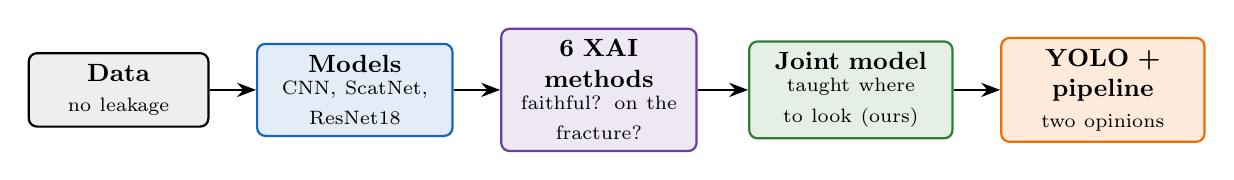
\begin{tikzpicture}[font=\small]
    \node[box, text width=2.0cm] (a) at (0,0) {\textbf{Data}\\\scriptsize no leakage};
    \node[bluebox, text width=2.2cm] (b) at (3.0,0) {\textbf{Models}\\\scriptsize CNN, ScatNet,\\ResNet18};
    \node[violetbox, text width=2.2cm] (c) at (6.1,0) {\textbf{6 XAI methods}\\\scriptsize faithful? on the\\fracture?};
    \node[greenbox, text width=2.3cm] (d) at (9.3,0) {\textbf{Joint model}\\\scriptsize taught where\\to look (ours)};
    \node[orangebox, text width=2.3cm] (e) at (12.5,0) {\textbf{YOLO + pipeline}\\\scriptsize two opinions};
    \draw[arr] (a)--(b); \draw[arr] (b)--(c); \draw[arr] (c)--(d); \draw[arr] (d)--(e);
  \end{tikzpicture}}
\end{frame}

\begin{frame}{The Data: FracAtlas, Without Leakage}
  \begin{columns}[T]
    \begin{column}{0.56\textwidth}
      \begin{figure}
        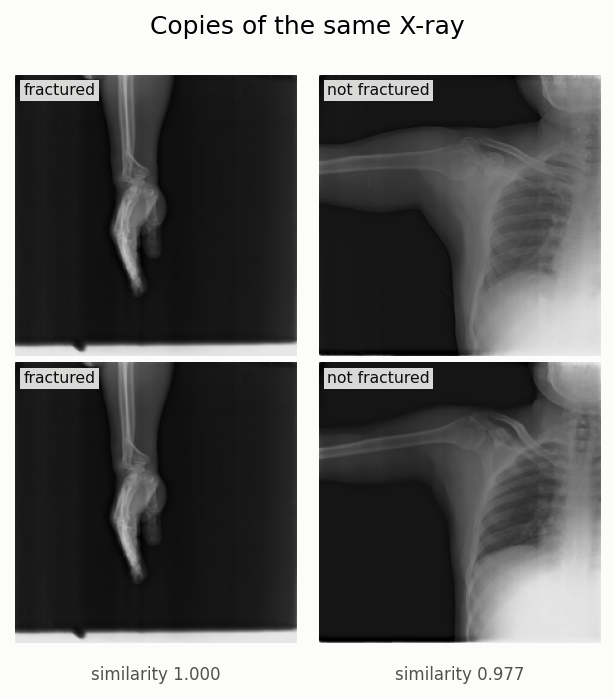
\includegraphics[width=\linewidth]{duplicates.png}
        \caption{Copies of the same X-ray (flipped, resized, brighter) found automatically.}
      \end{figure}
    \end{column}
    \begin{column}{0.42\textwidth}
      \small
      \begin{itemize}
        \item 4,083 X-rays; \textbf{717 fractured (1 in 6)}, 922 boxes.
        \item Grey, $224\times224$ (448 in our method), values in $[-1,1]$.
        \item \textbf{8.6\%} of the X-rays have a copy (158 groups): a split \textbf{keeps every group together}.
      \end{itemize}
      \centering\footnotesize
      \begin{tabular}{lccc}
        \toprule
        & X-rays & fractured & boxes \\
        \midrule
        train & 2,920 & 511 & 651 \\
        val & 577 & 102 & 136 \\
        test & 586 & 104 & 135 \\
        \bottomrule
      \end{tabular}
      \vspace{0.4em}

      \raggedright\small Always saying ``not fractured'' already scores \textbf{82.3\%}: look at \textbf{F1} and
      \textbf{fractures found}.
    \end{column}
  \end{columns}
\end{frame}

\begin{frame}{Three Feature Extractors, One Classifier}
  \centering
  \resizebox{\linewidth}{!}{%
  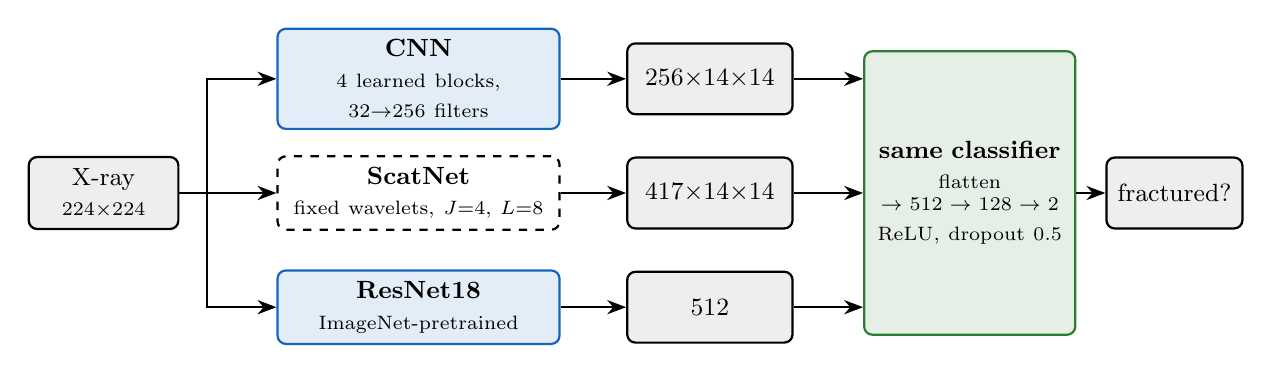
\begin{tikzpicture}[font=\small]
    \node[box, minimum width=1.9cm] (x) at (0,0) {X-ray\\\scriptsize $224{\times}224$};
    \node[bluebox, text width=3.3cm] (n1) at (4.0,1.45) {\textbf{CNN}\\\scriptsize 4 learned blocks, 32$\to$256 filters};
    \node[dashbox, text width=3.3cm] (n2) at (4.0,0) {\textbf{ScatNet}\\\scriptsize fixed wavelets, $J{=}4$, $L{=}8$};
    \node[bluebox, text width=3.3cm] (n3) at (4.0,-1.45) {\textbf{ResNet18}\\\scriptsize ImageNet-pretrained};
    \node[box, minimum width=2.1cm] (f1) at (7.7,1.45) {$256{\times}14{\times}14$};
    \node[box, minimum width=2.1cm] (f2) at (7.7,0) {$417{\times}14{\times}14$};
    \node[box, minimum width=2.1cm] (f3) at (7.7,-1.45) {512};
    \node[greenbox, text width=2.4cm, minimum height=3.6cm] (h) at (11.0,0) {\textbf{same classifier}\\[0.3em]\scriptsize flatten\\$\to512\to128\to2$\\ReLU, dropout 0.5};
    \node[box, minimum width=1.7cm] (o) at (13.6,0) {fractured?};
    \draw[arr] (x.east) -- ++(0.35,0) |- (n1.west); \draw[arr] (x)--(n2); \draw[arr] (x.east) -- ++(0.35,0) |- (n3.west);
    \draw[arr] (n1)--(f1); \draw[arr] (n2)--(f2); \draw[arr] (n3)--(f3);
    \draw[arr] (f1.east) -- (h.west|-f1); \draw[arr] (f2)--(h); \draw[arr] (f3.east) -- (h.west|-f3);
    \draw[arr] (h)--(o);
  \end{tikzpicture}}
  \vspace{0.4em}
  \begin{columns}[T]
    \begin{column}{0.32\textwidth}
      \small\textbf{CNN}: every filter \textbf{learned} from our 2,920 X-rays (first $7\times7$).
    \end{column}
    \begin{column}{0.32\textwidth}
      \small\textbf{ScatNet}: \textbf{nothing learned} before the classifier; stable to small deformations.
    \end{column}
    \begin{column}{0.32\textwidth}
      \small\textbf{ResNet18}: filters learned on \textbf{1.2M ImageNet} photos, then fine-tuned.
    \end{column}
  \end{columns}
  \vspace{0.3em}
  \footnotesize Only the classifier's \textbf{input size} differs (50,176 / 81,732 / 512). Weighted loss (1 in 6
  fractured), 20 epochs, 5-fold grouped CV.
\end{frame}

\begin{frame}{How ScatNet Works}
  \centering
  \resizebox{\linewidth}{!}{%
  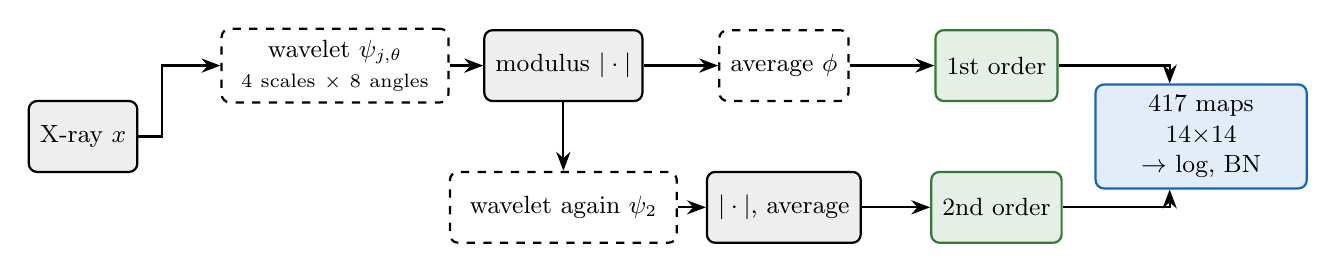
\begin{tikzpicture}[font=\small]
    \node[box] (x) at (0,0) {X-ray $x$};
    \node[dashbox, text width=2.6cm] (w1) at (3.2,0.9) {wavelet $\psi_{j,\theta}$\\\scriptsize 4 scales $\times$ 8 angles};
    \node[box] (m1) at (6.1,0.9) {modulus $|\cdot|$};
    \node[dashbox] (a1) at (8.9,0.9) {average $\phi$};
    \node[greenbox] (s1) at (11.6,0.9) {1st order};
    \node[dashbox, text width=2.6cm] (w2) at (6.1,-0.9) {wavelet again $\psi_2$};
    \node[box] (m2) at (8.9,-0.9) {$|\cdot|$, average};
    \node[greenbox] (s2) at (11.6,-0.9) {2nd order};
    \node[bluebox, text width=2.4cm] (o) at (14.2,0) {417 maps\\$14{\times}14$\\$\to$ log, BN};
    \draw[arr] (x.east) -- ++(0.3,0) |- (w1.west);
    \draw[arr] (w1)--(m1); \draw[arr] (m1)--(a1); \draw[arr] (a1)--(s1);
    \draw[arr] (m1)--(w2); \draw[arr] (w2)--(m2); \draw[arr] (m2)--(s2);
    \draw[arr] (s1.east) -| ([xshift=-4mm]o.north); \draw[arr] (s2.east) -| ([xshift=-4mm]o.south);
  \end{tikzpicture}}
  \vspace{0.5em}
  \begin{columns}[T]
    \begin{column}{0.48\textwidth}
      \textbf{The idea} (Bruna \& Mallat, 2013)
      \begin{itemize}\small
        \item A CNN with \textbf{fixed} filters: Morlet wavelets at every scale and angle.
        \item Modulus + averaging $\Rightarrow$ \textbf{stable to small shifts and deformations}.
        \item 1 + 32 + 384 = \textbf{417} coefficient maps (Kymatio, $J{=}4$, $L{=}8$).
      \end{itemize}
    \end{column}
    \begin{column}{0.48\textwidth}
      \textbf{For fractures}
      \begin{itemize}\small
        \item $+$ No filters to learn: good with \textbf{little data}.
        \item $-$ A small break \textbf{is} a small deformation: the averaging blurs exactly what we need.
        \item $-$ Every coefficient is kept: the classifier has 41.9M parameters.
      \end{itemize}
    \end{column}
  \end{columns}
\end{frame}

\begin{frame}{CNN vs ScatNet (+ ResNet18): Results}
  \begin{columns}[T]
    \begin{column}{0.5\textwidth}
      \centering\footnotesize
      \begin{tabular}{lccc}
        \toprule
        & \textbf{CNN} & \textbf{ScatNet} & \textbf{ResNet18} \\
        \midrule
        CV accuracy & $73.0{\pm}9.0$ & $77.5{\pm}2.9$ & $\mathbf{89.0{\pm}1.0}$ \\
        CV F1 & $35.7{\pm}13.0$ & $38.0{\pm}2.6$ & $\mathbf{66.6{\pm}2.7}$ \\
        \midrule
        test accuracy & 80.9 & 80.0 & \textbf{91.5} \\
        test F1 & 23.3 & 31.6 & \textbf{73.7} \\
        fractures found & 16\% & 26\% & \textbf{67\%} \\
        AUC & 68.6 & 72.7 & \textbf{91.2} \\
        parameters & 26.1M & 41.9M & 11.5M \\
        \bottomrule
      \end{tabular}
      \vspace{0.6em}

      \raggedright\small
      McNemar: CNN $\approx$ ScatNet ($p=0.55$); ResNet18 beats both ($p<0.001$).
    \end{column}
    \begin{column}{0.48\textwidth}
      \small
      \textbf{Why CNN and ScatNet fail}
      \begin{itemize}
        \item Both \textbf{underfit} (loss stuck at 0.6) and stay \textbf{below} the 82.3\% of ``never fractured''.
        \item Only 511 fractured X-rays; a fracture is 1--2 px wide at 224 px.
        \item Flattening a $14{\times}14$ grid: 26--42M parameters in the classifier.
      \end{itemize}
      \textbf{Why ResNet18 wins}
      \begin{itemize}
        \item Pretrained edge and texture detectors that 2,920 X-rays cannot teach.
        \item It overfits after $\approx$10 epochs: the best val epoch is kept.
      \end{itemize}
    \end{column}
  \end{columns}
\end{frame}

\begin{frame}{Learning Curves and Filters}
  \begin{columns}[T]
    \begin{column}{0.58\textwidth}
      \begin{figure}
        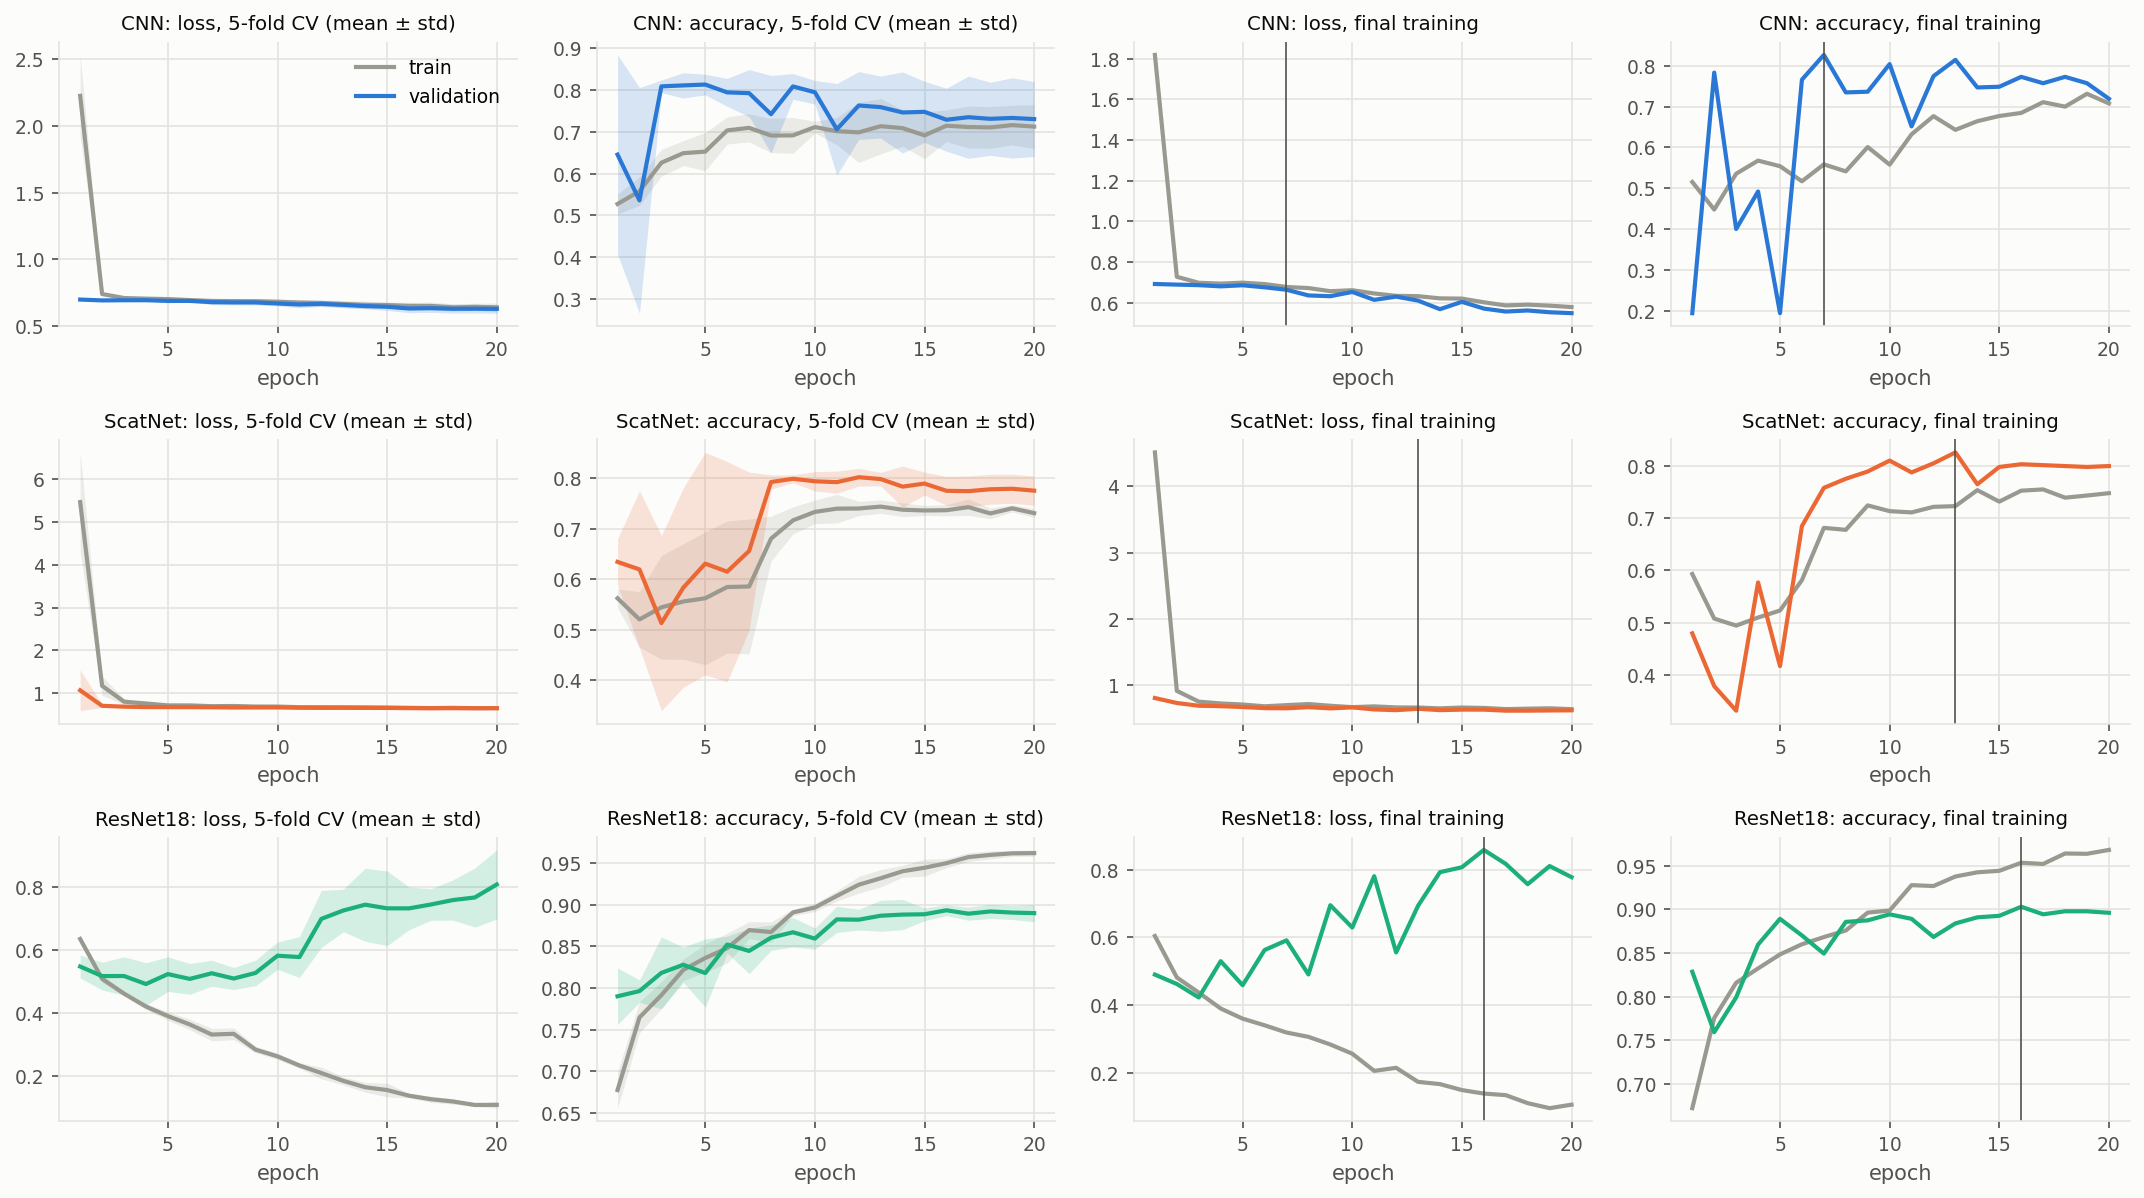
\includegraphics[width=\linewidth]{learning_curves.png}
        \caption{Train (grey) and validation (colour): 5-fold CV and final training.}
      \end{figure}
    \end{column}
    \begin{column}{0.4\textwidth}
      \begin{figure}
        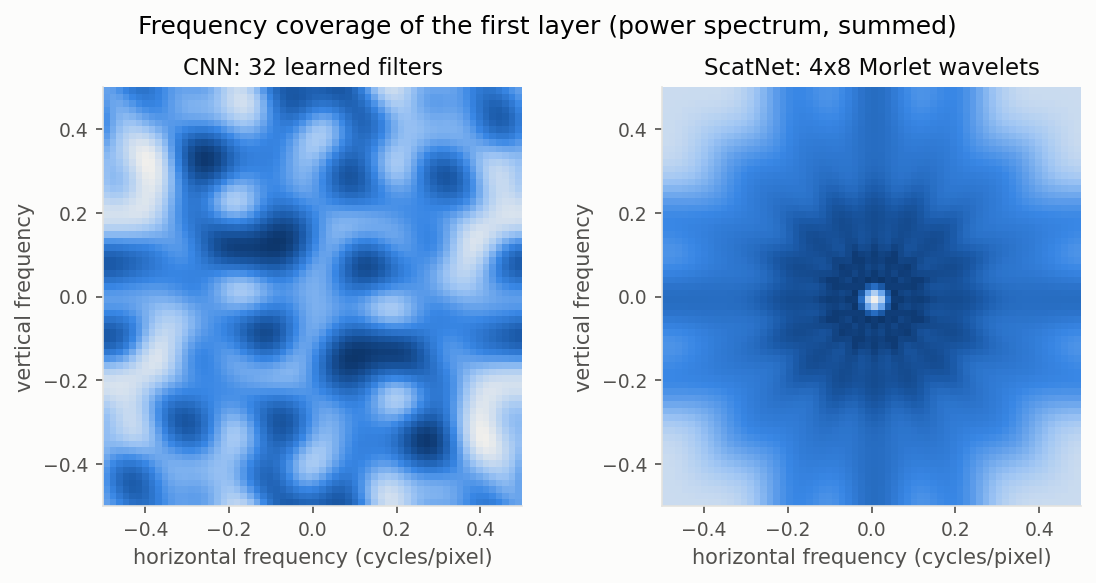
\includegraphics[width=0.9\linewidth]{frequency_coverage.png}
        \caption{First-layer filters in frequency.}
      \end{figure}
      \vspace{-0.5em}
      \footnotesize
      \begin{itemize}
        \item CNN: noisy learned filters, \textbf{uneven} coverage.
        \item ScatNet: clean wavelets, \textbf{every} scale and angle.
        \item Clean filters are not enough: ScatNet lacks a \textbf{learned} hierarchy above them.
      \end{itemize}
    \end{column}
  \end{columns}
\end{frame}

\begin{frame}{Six XAI Methods: How Each One Works}
  \centering\footnotesize
  \renewcommand{\arraystretch}{1.25}\setlength{\tabcolsep}{4pt}
  \begin{tabular}{>{\raggedright\arraybackslash\bfseries}p{2.3cm}>{\raggedright\arraybackslash}p{6.3cm}>{\raggedright\arraybackslash}p{3.0cm}c}
    \toprule
    & \textbf{how it works} & \textbf{strength / weakness} & \textbf{s/X-ray} \\
    \midrule
    Saliency & $|\partial z_c/\partial x|$: score change for a tiny change of each pixel & fast / noisy, saturates & 0.015 \\
    Integrated Gradients & gradients averaged on the path black $\to$ $x$, times $(x-x')$; sums to $z_c(x)-z_c(x')$ & complete / slower & 0.194 \\
    Guided Backprop & gradient, negative signals stopped at every ReLU & sharp / like an edge detector & 0.010 \\
    Grad-CAM & last conv layer: channels weighted by their mean gradient, ReLU & class-specific / coarse; \textbf{not on ScatNet} & 0.005 \\
    Occlusion & slide a black $16{\times}16$ window, record the score drop & honest / slow & 0.767 \\
    LIME & switch random $16{\times}16$ patches off, fit a ridge regression & honest / random, slowest & 1.377 \\
    \bottomrule
  \end{tabular}
  \vspace{0.6em}

  \raggedright\small
  \textbf{Gradient} methods ask ``what if this pixel changed a little?''; \textbf{perturbation} methods (Occlusion, LIME)
  really \textbf{remove} parts of the X-ray (black = removed).
  Grad-CAM needs a learned convolutional layer, which ScatNet does not have.
\end{frame}

\begin{frame}{The Six Methods on the Same X-rays}
  \begin{columns}[T]
    \begin{column}{0.5\textwidth}
      \begin{figure}
        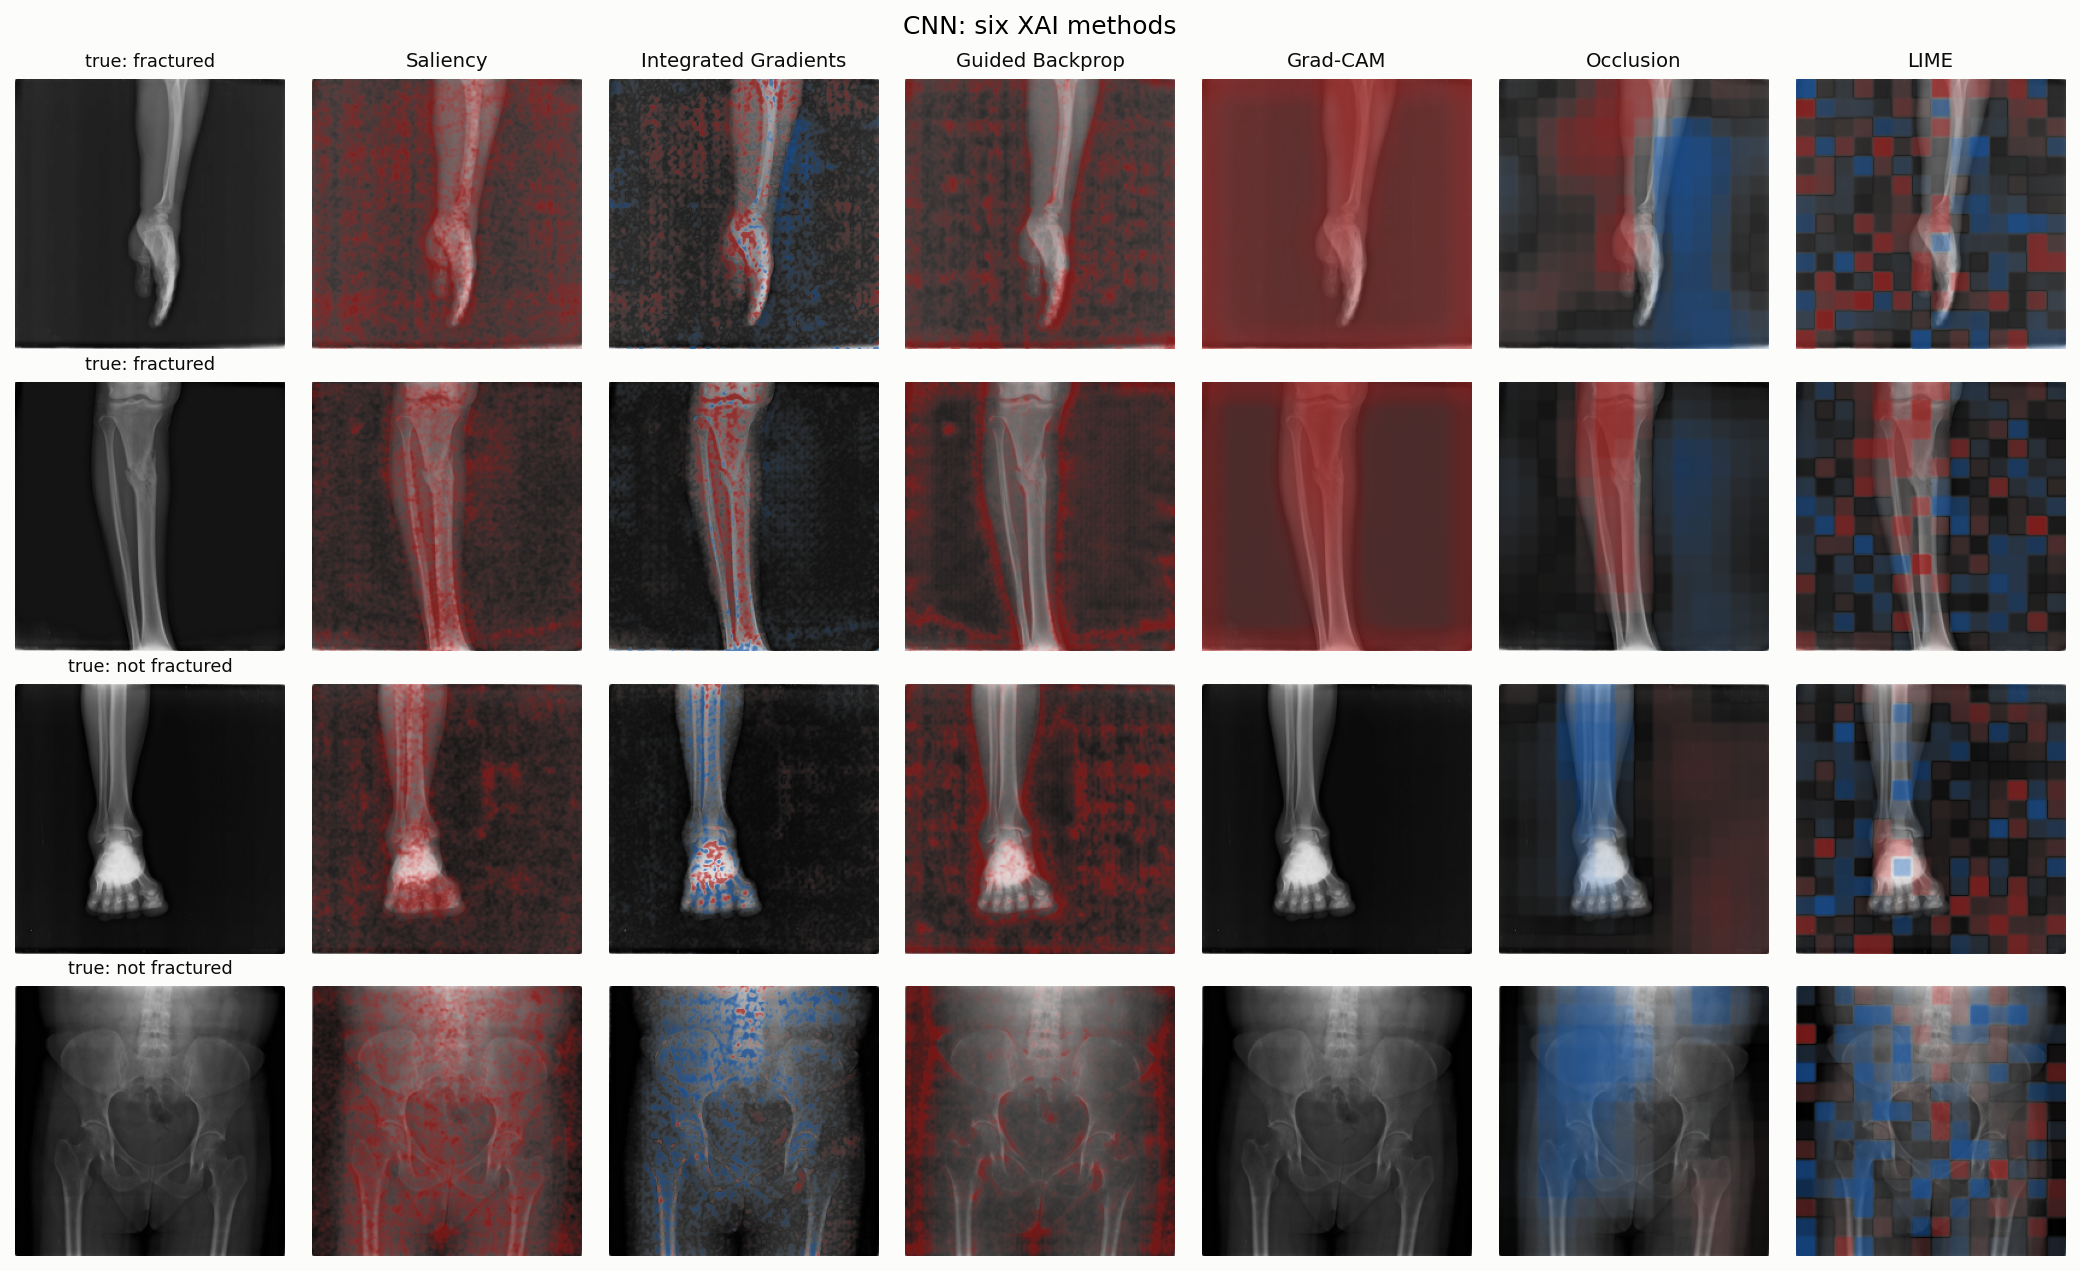
\includegraphics[width=\linewidth]{xai_cnn.png}
        \caption{CNN: 2 fractured, 2 healthy (red = for, blue = against).}
      \end{figure}
    \end{column}
    \begin{column}{0.5\textwidth}
      \begin{figure}
        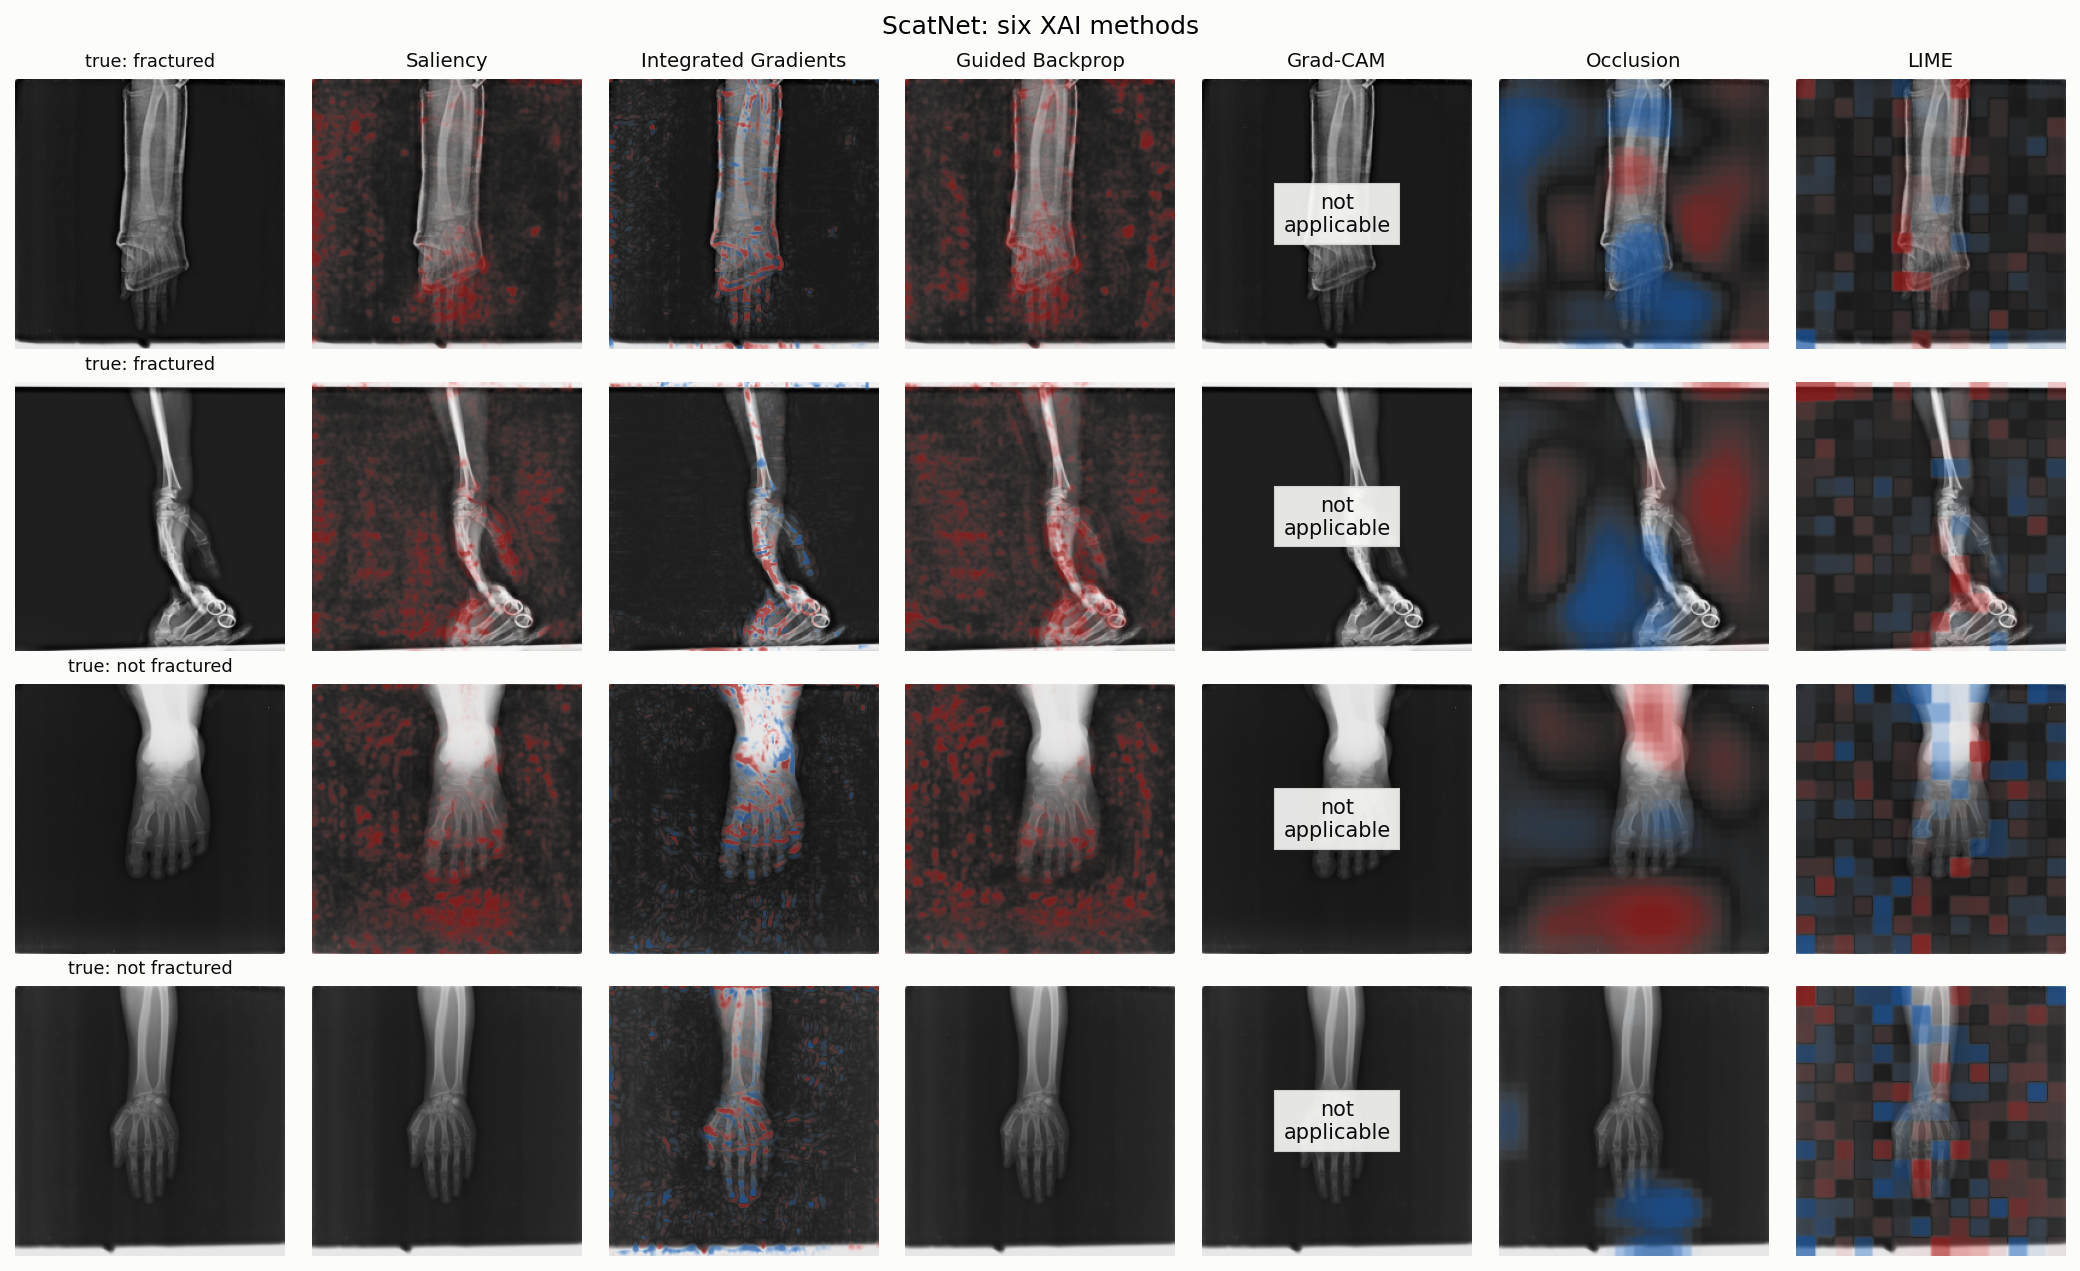
\includegraphics[width=\linewidth]{xai_scatnet.png}
        \caption{ScatNet: Grad-CAM not applicable.}
      \end{figure}
    \end{column}
  \end{columns}
  \small
  \begin{itemize}
    \item The six maps are \textbf{visibly different}: there is no single ``true'' explanation.
    \item CNN's Grad-CAM covers large areas; ScatNet's maps are spread all over the image.
  \end{itemize}
\end{frame}

\begin{frame}{Occlusion, Written From Scratch}
  \begin{columns}[T]
    \begin{column}{0.44\textwidth}
      \scriptsize
      \begin{algorithmic}
        \Require model $f$, X-ray $x$, class $c$, window $w{=}16$, stride $s{=}8$
        \State $z \gets f(x)_c$;\ \ $A\gets 0$;\ \ $N\gets 0$
        \For{every window position $(i,j)$, in batches}
          \State $\hat x \gets x$ with the window set to black
          \State $A[\text{window}] \mathrel{+}= z - f(\hat x)_c$
          \State $N[\text{window}] \mathrel{+}= 1$
        \EndFor
        \State \Return $A / N$ \Comment{mean drop per pixel}
      \end{algorithmic}
      \vspace{0.5em}
      \small
      \begin{itemize}
        \item Plain PyTorch, all positions scored in batches.
        \item Same answer as Captum on all three models: Pearson $r=1.000$, largest difference
              $\mathbf{8.6\cdot10^{-6}}$.
      \end{itemize}
    \end{column}
    \begin{column}{0.54\textwidth}
      \begin{figure}
        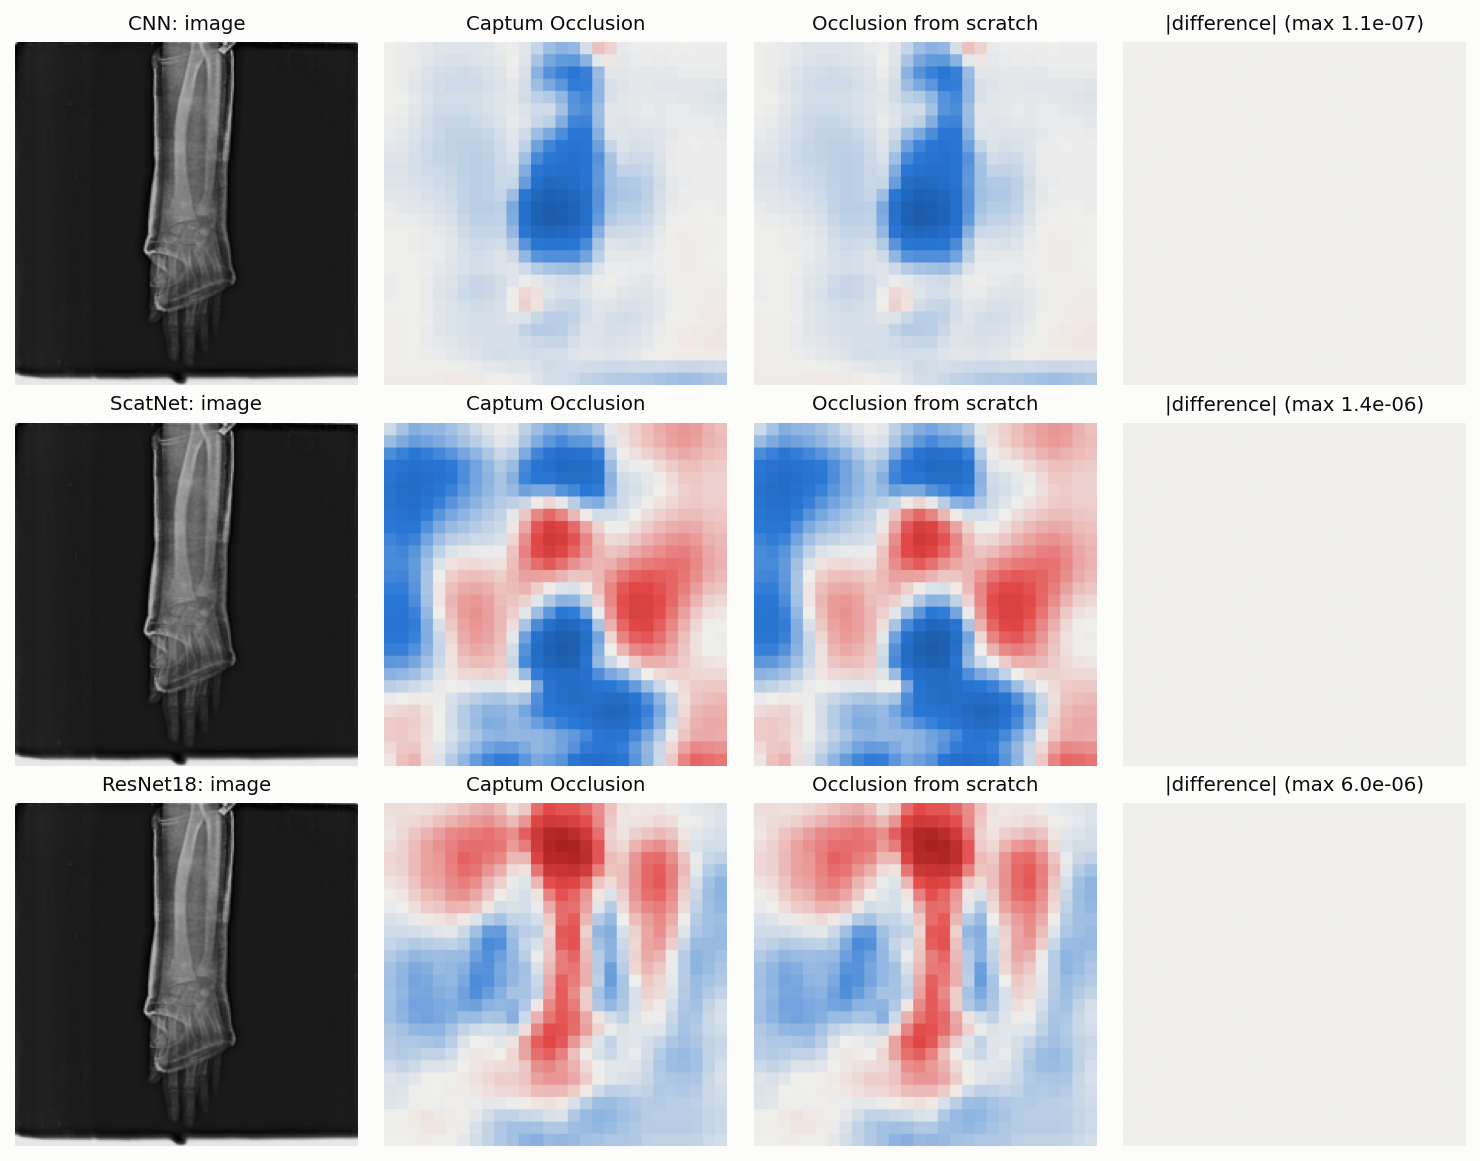
\includegraphics[width=\linewidth]{occlusion_scratch_vs_captum.png}
        \caption{Our Occlusion, Captum's, and their difference.}
      \end{figure}
    \end{column}
  \end{columns}
\end{frame}

\begin{frame}{Is the Map Faithful? The Deletion Test}
  \begin{columns}[T]
    \begin{column}{0.5\textwidth}
      \small
      Remove the \textbf{most important} $16{\times}16$ patches \textbf{first} and follow the class probability:
      a faithful map makes it fall fast (low area). A random order is the reference.
      \vspace{0.5em}

      \centering\footnotesize
      \begin{tabular}{lccc}
        \toprule
        \textbf{deletion AUC} & \textbf{CNN} & \textbf{ScatNet} & \textbf{ResNet18} \\
        \midrule
        Saliency & 0.530 & 0.573 & 0.663 \\
        Integrated Grad. & 0.510 & 0.572 & 0.637 \\
        Guided Backprop & 0.511 & \textbf{0.552} & 0.555 \\
        Grad-CAM & \textbf{0.497} & n/a & 0.580 \\
        Occlusion & 0.572 & 0.588 & 0.562 \\
        LIME & 0.528 & 0.554 & \textbf{0.496} \\
        \midrule
        random & 0.570 & 0.576 & 0.700 \\
        \bottomrule
      \end{tabular}
    \end{column}
    \begin{column}{0.48\textwidth}
      \small
      \textbf{The winner depends on the model}
      \begin{itemize}
        \item \textbf{CNN}: Grad-CAM. The last conv layer of a small CNN is where it decides.
        \item \textbf{ScatNet}: all close to random. Its evidence is spread over hundreds of wavelet coefficients;
              no small region matters alone.
        \item \textbf{ResNet18}: LIME. It does what the test does: removes patches.
        \item Saliency and IG are the least faithful on ResNet18: gradients are local and saturate in a deep net.
      \end{itemize}
    \end{column}
  \end{columns}
\end{frame}

\begin{frame}{Does the Map Point at the Fracture?}
  \centering
  \resizebox{\linewidth}{!}{%
  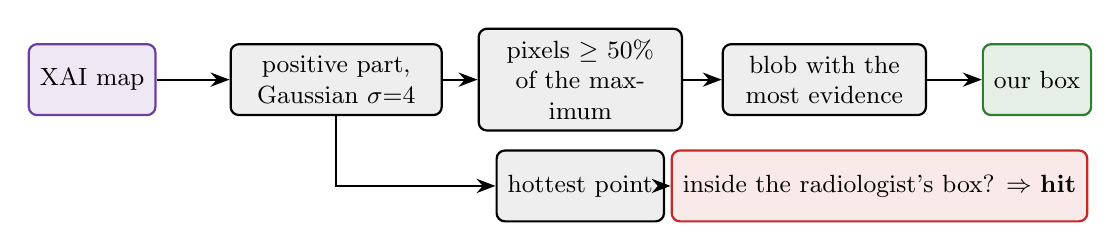
\begin{tikzpicture}[font=\small]
    \node[violetbox] (m) at (0,0) {XAI map};
    \node[box, text width=2.4cm] (a) at (3.1,0) {positive part,\\Gaussian $\sigma{=}4$};
    \node[box, text width=2.3cm] (b) at (6.2,0) {pixels $\ge$ 50\%\\of the maximum};
    \node[box, text width=2.3cm] (c) at (9.3,0) {blob with the\\most evidence};
    \node[greenbox] (d) at (12.0,0) {our box};
    \node[box] (p) at (6.2,-1.35) {hottest point};
    \node[redbox] (h) at (10.0,-1.35) {inside the radiologist's box? $\Rightarrow$ \textbf{hit}};
    \draw[arr] (m)--(a); \draw[arr] (a)--(b); \draw[arr] (b)--(c); \draw[arr] (c)--(d);
    \draw[arr] (a.south) |- (p.west); \draw[arr] (p)--(h);
  \end{tikzpicture}}
  \vspace{0.4em}
  \begin{columns}[T]
    \begin{column}{0.42\textwidth}
      \centering\scriptsize\setlength{\tabcolsep}{3pt}
      \begin{tabular}{lccc}
        \toprule
        \textbf{hit rate (\%)} & CNN & ScatNet & ResNet18 \\
        \midrule
        Saliency & 3.8 & 0.0 & 3.8 \\
        Integrated Grad. & 2.9 & 2.9 & \textbf{23.1} \\
        Guided Backprop & 3.8 & 0.0 & 4.8 \\
        Grad-CAM & 0.0 & n/a & 9.6 \\
        Occlusion & 3.8 & 3.8 & 6.7 \\
        LIME & 0.0 & 0.0 & 1.0 \\
        \bottomrule
      \end{tabular}
      \\[0.2em]\scriptsize 104 fractured test X-rays; random point: 1\%.
    \end{column}
    \begin{column}{0.54\textwidth}
      \small
      \textbf{Rarely.} Best: Integrated Gradients on ResNet18, \textbf{23\%}. Why so low?
      \begin{itemize}
        \item The boxes are \textbf{tiny} (1\% of the image); fractures are 1--2 px at 224 px.
        \item A third of the fractures are \textbf{missed} by the model.
        \item The model also uses \textbf{shortcuts} (plates, casts), and the faithful maps honestly show them.
      \end{itemize}
      $\Rightarrow$ Faithful maps are not enough: the \textbf{model} must look at the fracture.
    \end{column}
  \end{columns}
\end{frame}

% ════════════════════════════════════════════════════════════════════════════════════════════════
\partslide{II}{Teach the Model Where to Look}{One network that classifies, detects, and is trained on its own explanation}
\section{Our method}

\begin{frame}{A First Attempt That Failed}
  \begin{columns}[T]
    \begin{column}{0.5\textwidth}
      \centering
      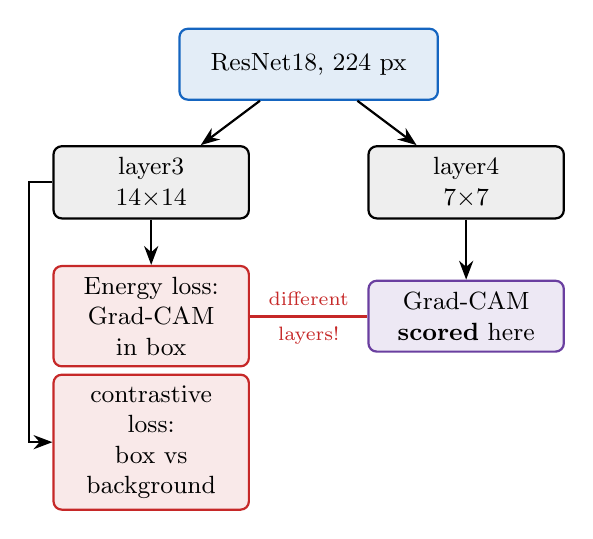
\begin{tikzpicture}[font=\small]
        \node[bluebox, text width=3.0cm] (r) at (0,0) {ResNet18, 224 px};
        \node[box, text width=2.2cm] (l3) at (-2.0,-1.5) {layer3\\$14{\times}14$};
        \node[box, text width=2.2cm] (l4) at (2.0,-1.5) {layer4\\$7{\times}7$};
        \node[redbox, text width=2.2cm] (e) at (-2.0,-3.2) {Energy loss:\\Grad-CAM in box};
        \node[redbox, text width=2.2cm] (s) at (-2.0,-4.8) {contrastive loss:\\box vs background};
        \node[violetbox, text width=2.2cm] (g) at (2.0,-3.2) {Grad-CAM\\\textbf{scored} here};
        \draw[arr] (r) -- (l3); \draw[arr] (r) -- (l4); \draw[arr] (l3)--(e); \draw[arr] (l4)--(g);
        \draw[arr] (l3.west) -- ++(-0.3,0) |- (s.west);
        \draw[myred, very thick] (e.east) -- node[lab, text=myred, above]{different} node[lab, text=myred, below]{layers!} (g.west);
      \end{tikzpicture}
    \end{column}
    \begin{column}{0.48\textwidth}
      \small
      \textbf{Result}: Grad-CAM hit rate 10.6\% $\to$ 10.6\%, and \textbf{5.8\%} with the contrastive loss.
      \vspace{0.4em}

      \textbf{Three reasons, three lessons}
      \begin{enumerate}
        \item Trained on layer3, \textbf{scored on layer4} $\Rightarrow$ score the layer you train.
        \item Grad-CAM's ReLU let the map \textbf{collapse to zero}: no gradient left $\Rightarrow$ use a smooth target
              (softmax).
        \item The contrastive loss hit its \textbf{lowest value at once}: a box on bone vs black background is trivially
              different $\Rightarrow$ compare things that are hard to tell apart.
      \end{enumerate}
    \end{column}
  \end{columns}
\end{frame}

\begin{frame}{Our Joint Model}
  \centering
  \resizebox{\linewidth}{!}{%
  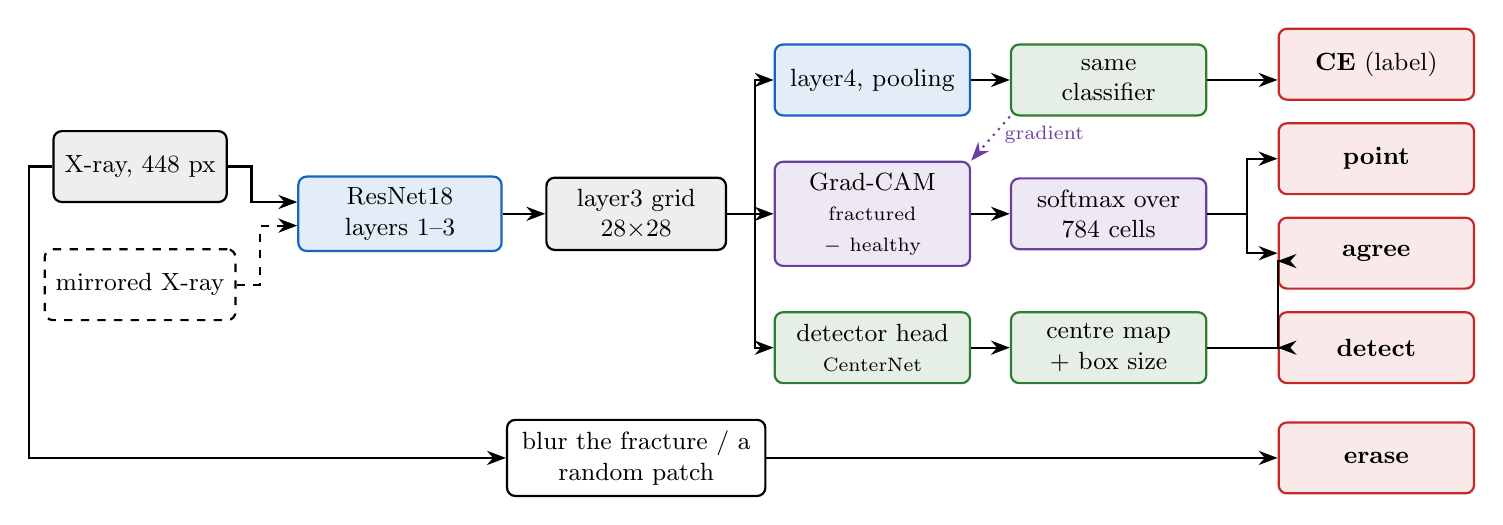
\begin{tikzpicture}[font=\small]
    \node[box, minimum width=2.2cm] (x) at (0,0.6) {X-ray, 448 px};
    \node[dashbox, minimum width=2.2cm] (xm) at (0,-0.9) {mirrored X-ray};
    \node[bluebox, text width=2.3cm] (bb) at (3.3,0) {ResNet18\\layers 1--3};
    \node[box, text width=2.0cm] (g) at (6.3,0) {layer3 grid\\$28{\times}28$};
    \node[bluebox, text width=2.2cm] (l4) at (9.3,1.7) {layer4, pooling};
    \node[greenbox, text width=2.2cm] (cl) at (12.3,1.7) {same\\classifier};
    \node[violetbox, text width=2.2cm] (gc) at (9.3,0) {Grad-CAM\\\scriptsize fractured $-$ healthy};
    \node[violetbox, text width=2.2cm] (sm) at (12.3,0) {softmax over\\784 cells};
    \node[greenbox, text width=2.2cm] (dh) at (9.3,-1.7) {detector head\\\scriptsize CenterNet};
    \node[greenbox, text width=2.2cm] (cm) at (12.3,-1.7) {centre map\\+ box size};
    \node[redbox, text width=2.2cm] (lce) at (15.7,1.9) {\textbf{CE} (label)};
    \node[redbox, text width=2.2cm] (lp) at (15.7,0.7) {\textbf{point}};
    \node[redbox, text width=2.2cm] (la) at (15.7,-0.5) {\textbf{agree}};
    \node[redbox, text width=2.2cm] (ld) at (15.7,-1.7) {\textbf{detect}};
    \node[box, fill=white, text width=3.0cm] (bl) at (6.3,-3.1) {blur the fracture / a\\random patch};
    \node[redbox, text width=2.2cm] (le) at (15.7,-3.1) {\textbf{erase}};
    \draw[arr] (x.east) -- ++(0.3,0) |- ([yshift=1.5mm]bb.west);
    \draw[arr, dashed] (xm.east) -- ++(0.3,0) |- ([yshift=-1.5mm]bb.west);
    \draw[arr] (bb)--(g);
    \draw[arr] (g.east) -- ++(0.35,0) |- (l4.west); \draw[arr] (g)--(gc); \draw[arr] (g.east) -- ++(0.35,0) |- (dh.west);
    \draw[arr] (l4)--(cl); \draw[arr] (gc)--(sm); \draw[arr] (dh)--(cm);
    \draw[arr] (cl.east) -- (lce.west|-cl); \draw[arr] (sm.east) -- ++(0.5,0) |- (lp.west); \draw[arr] (sm.east) -- ++(0.5,0) |- (la.west);
    \draw[arr] (cm.east) -- ++(0.9,0) |- ([yshift=-1mm]la.west); \draw[arr] (cm.east) -- ++(0.9,0) |- (ld.west);
    \draw[arr] (x.west) -- ++(-0.3,0) |- (bl.west); \draw[arr] (bl)--(le);
    \draw[arr, myviolet, dotted] (cl.south west) -- node[lab, text=myviolet, right, pos=0.4]{gradient} (gc.north east);
  \end{tikzpicture}}
  \vspace{0.2em}
  \begin{columns}[T]
    \begin{column}{0.49\textwidth}
      \small
      \begin{itemize}
        \item \textbf{448 px}: four times the pixels, thin fractures survive.
        \item One \textbf{shared grid} of 16-px cells feeds three heads: classifier, detector, Grad-CAM.
      \end{itemize}
    \end{column}
    \begin{column}{0.49\textwidth}
      \small
      \begin{itemize}
        \item Grad-CAM is computed \textbf{during training}, on the layer that is scored.
        \item \textbf{A}: CE only.\quad \textbf{B}: + detect.\quad \textbf{C}: all five (ours).
      \end{itemize}
    \end{column}
  \end{columns}
\end{frame}

\begin{frame}{The Five Losses: What Each Does and Why}
  \centering\footnotesize
  \renewcommand{\arraystretch}{1.3}\setlength{\tabcolsep}{4pt}
  \begin{tabular}{>{\raggedright\arraybackslash\bfseries}p{1.4cm}>{\raggedright\arraybackslash}p{5.6cm}>{\raggedright\arraybackslash}p{6.1cm}}
    \toprule
    & \textbf{what it asks} & \textbf{why it should help} \\
    \midrule
    CE & the right label (batches half fractured) & the classification task \\
    detect & CenterNet: a peak at the fracture centre + the box size & multi-task: the shared grid must learn \textbf{where} fractures are \\
    point & $-\log\sum_{i\in\text{box}}p_i$, \ $p=$ softmax of Grad-CAM & a smooth version of the hit rate; the softmax never loses its gradient \\
    agree & $\mathrm{JS}(p,q_{\text{detector}})+\mathrm{JS}(p,\mathrm{flip}(p_{\text{mirror}}))$ & SimCLR-like: two views must point at the same place; updates \textbf{both} heads \\
    erase & blurred fracture $\Rightarrow$ ``healthy''; blurred random patch $\Rightarrow$ still ``fractured'' & a map can move without the reasoning; the \textbf{decision} must follow the fracture \\
    \bottomrule
  \end{tabular}
  \vspace{0.6em}
  \[
    \mathcal{L}=\mathrm{CE}+\lambda_d\,\mathcal{L}_{\text{det}}+r(t)\big[\lambda_p\mathcal{L}_{\text{point}}
    +\lambda_a\mathcal{L}_{\text{agree}}+\lambda_e\mathcal{L}_{\text{erase}}\big],\qquad
    \lambda_d{=}1,\ \lambda_{p,a,e}{=}0.5
  \]
  \small The explanation losses start after a 2-epoch warm-up $r(t)$. Same data, budget and seed for A, B and C.
\end{frame}

\begin{frame}{A vs B vs C: Accuracy}
  \begin{columns}[T]
    \begin{column}{0.55\textwidth}
      \centering\footnotesize
      \begin{tabular}{lccccc}
        \toprule
        & \textbf{accuracy} & \textbf{F1} & \textbf{found} & \textbf{false al.} & \textbf{AUC} \\
        \midrule
        ResNet18, 224 & 91.5 & 73.7 & 67\% & 16 & 91.2 \\
        A: separate & 93.3 & 81.0 & 80\% & 18 & 94.4 \\
        B: + detector & \textbf{94.2} & \textbf{82.3} & 76\% & \textbf{9} & 94.3 \\
        C: + XAI losses & 93.0 & 80.4 & \textbf{81\%} & 21 & \textbf{95.2} \\
        \bottomrule
      \end{tabular}
      \\[0.3em]\scriptsize 586 test X-rays; threshold chosen on val F1.
      \begin{figure}
        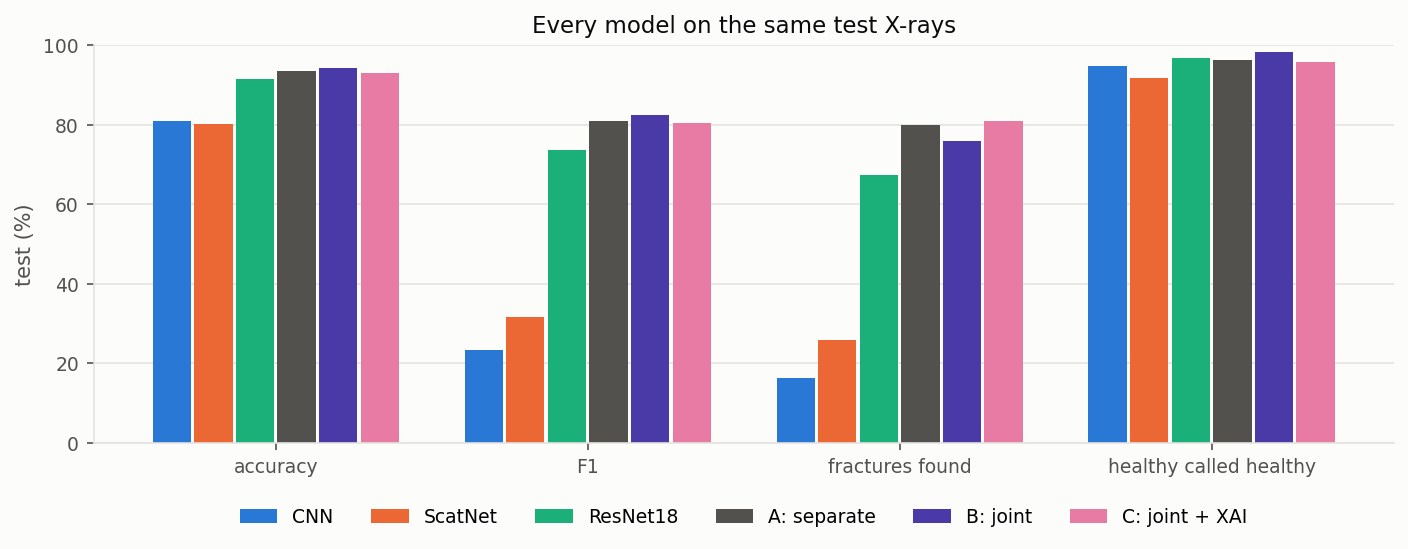
\includegraphics[width=0.92\linewidth]{final_scoreboard.png}
      \end{figure}
    \end{column}
    \begin{column}{0.43\textwidth}
      \small
      \begin{itemize}
        \item \textbf{448 px} already helps: A finds 80\% of the fractures vs 67\%.
        \item A, B and C are \textbf{within each other's confidence intervals} (about $\pm2$ points).
        \item A second full run gave 91.1, 93.3, 93.9\%: one-point gaps are noise.
      \end{itemize}
      \vspace{0.3em}
      \colorbox{myblue!10}{\parbox{0.92\linewidth}{\small Our method does not change \textbf{how often} the model is
      right. It changes \textbf{why}: next slides.}}
    \end{column}
  \end{columns}
\end{frame}

\begin{frame}{A vs B vs C: Where Do the Explanations Point?}
  \begin{columns}[T]
    \begin{column}{0.55\textwidth}
      \begin{figure}
        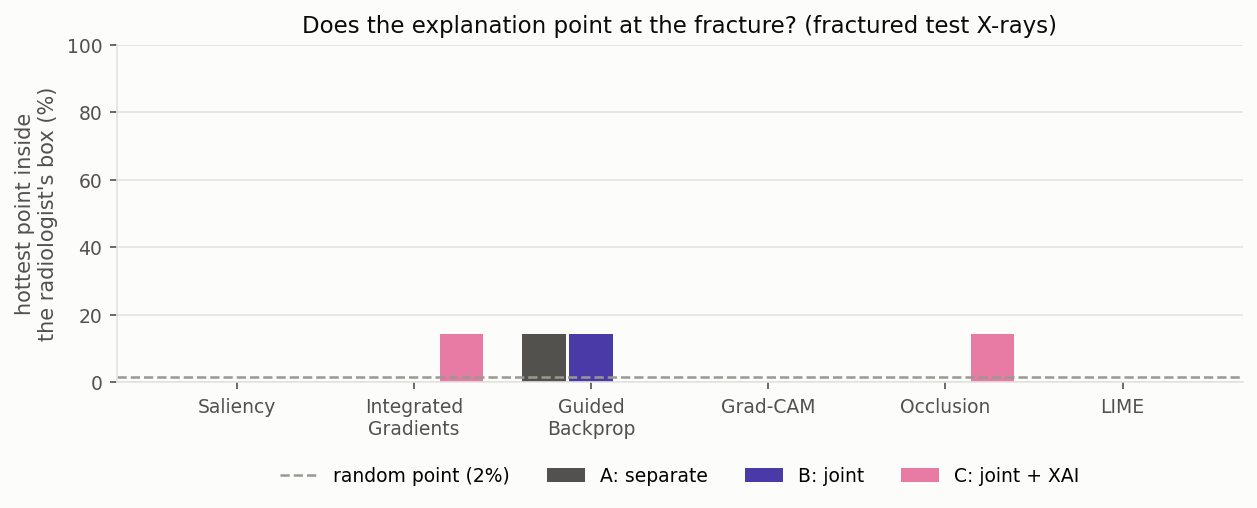
\includegraphics[width=\linewidth]{joint_localization.png}
        \caption{Hit rate of the six methods, 104 fractured test X-rays.}
      \end{figure}
    \end{column}
    \begin{column}{0.43\textwidth}
      \centering\footnotesize
      \begin{tabular}{lccc}
        \toprule
        & A & C & $p$ (A vs C) \\
        \midrule
        Grad-CAM & 35 & \textbf{67} & $<$0.001 \\
        Guided Backprop & 33 & \textbf{52} & 0.0001 \\
        Occlusion & 32 & 43 & 0.050 \\
        Integrated Grad. & 54 & 62 & 0.077 \\
        Saliency & 40 & 49 & 0.136 \\
        LIME & 16 & 24 & 0.115 \\
        \bottomrule
      \end{tabular}
      \vspace{0.3em}
      \small
      \begin{itemize}
        \item \textbf{B}: the detector alone lifts every method (mean 35 $\to$ 48\%).
        \item \textbf{C}: Grad-CAM \textbf{doubles} (36 $\to$ 70 of 104 X-rays).
        \item Only Grad-CAM is in the loss, yet every method improves.
      \end{itemize}
    \end{column}
  \end{columns}
\end{frame}

\begin{frame}{Is It Real? Blur the Fracture}
  \begin{columns}[T]
    \begin{column}{0.52\textwidth}
      \begin{figure}
        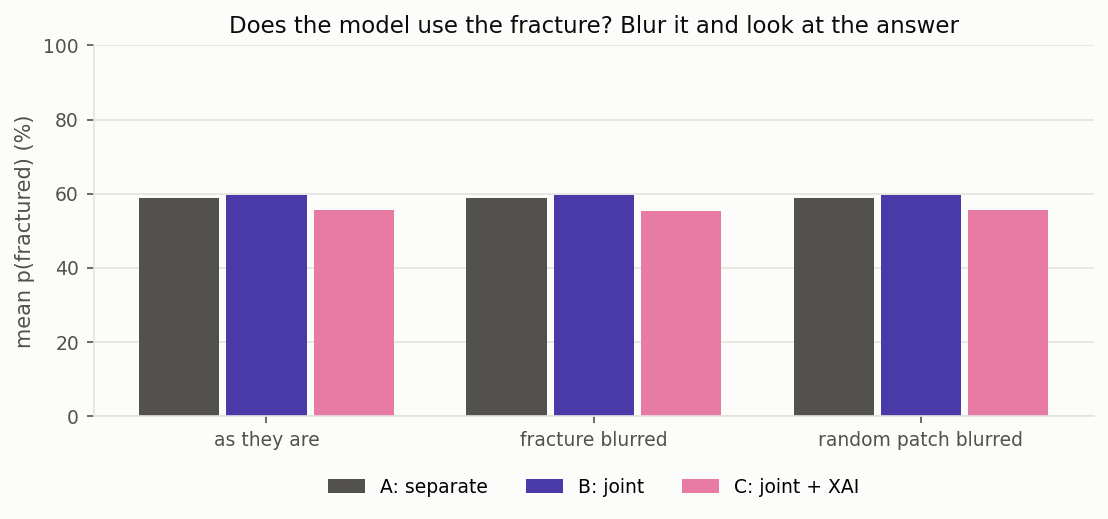
\includegraphics[width=\linewidth]{erase_test.png}
        \caption{Mean $p(\text{fractured})$ of the fractured test X-rays.}
      \end{figure}
      \centering\footnotesize
      \begin{tabular}{lccc}
        \toprule
        & as they are & fracture blurred & random patch \\
        \midrule
        A & 80.6 & 84.4 & 80.9 \\
        B & 77.0 & 47.7 & 77.7 \\
        C & 83.7 & \textbf{2.5} & 79.4 \\
        \bottomrule
      \end{tabular}
    \end{column}
    \begin{column}{0.46\textwidth}
      \small
      \begin{itemize}
        \item \textbf{A ignores the fracture}: blur it and its answer does not change.
        \item \textbf{C decides from the fracture}: blur it and $p$ falls to 2.5\%; blur an equal patch elsewhere and it
              stays at 79\%.
        \item So the better maps are \textbf{not cosmetic}: the decision moved with them.
        \item Faithfulness is kept: mean deletion AUC 0.55 (A), 0.52 (B), 0.54 (C).
      \end{itemize}
      \vspace{0.2em}
      \footnotesize C is trained with this blur on other X-rays; the random-patch control and the five methods outside
      its loss are the independent evidence. Same picture in a second full run (blur drop 81 points).
    \end{column}
  \end{columns}
\end{frame}

\begin{frame}{Random Test X-rays (Not Picked by Hand)}
  \begin{columns}[T]
    \begin{column}{0.4\textwidth}
      \begin{figure}
        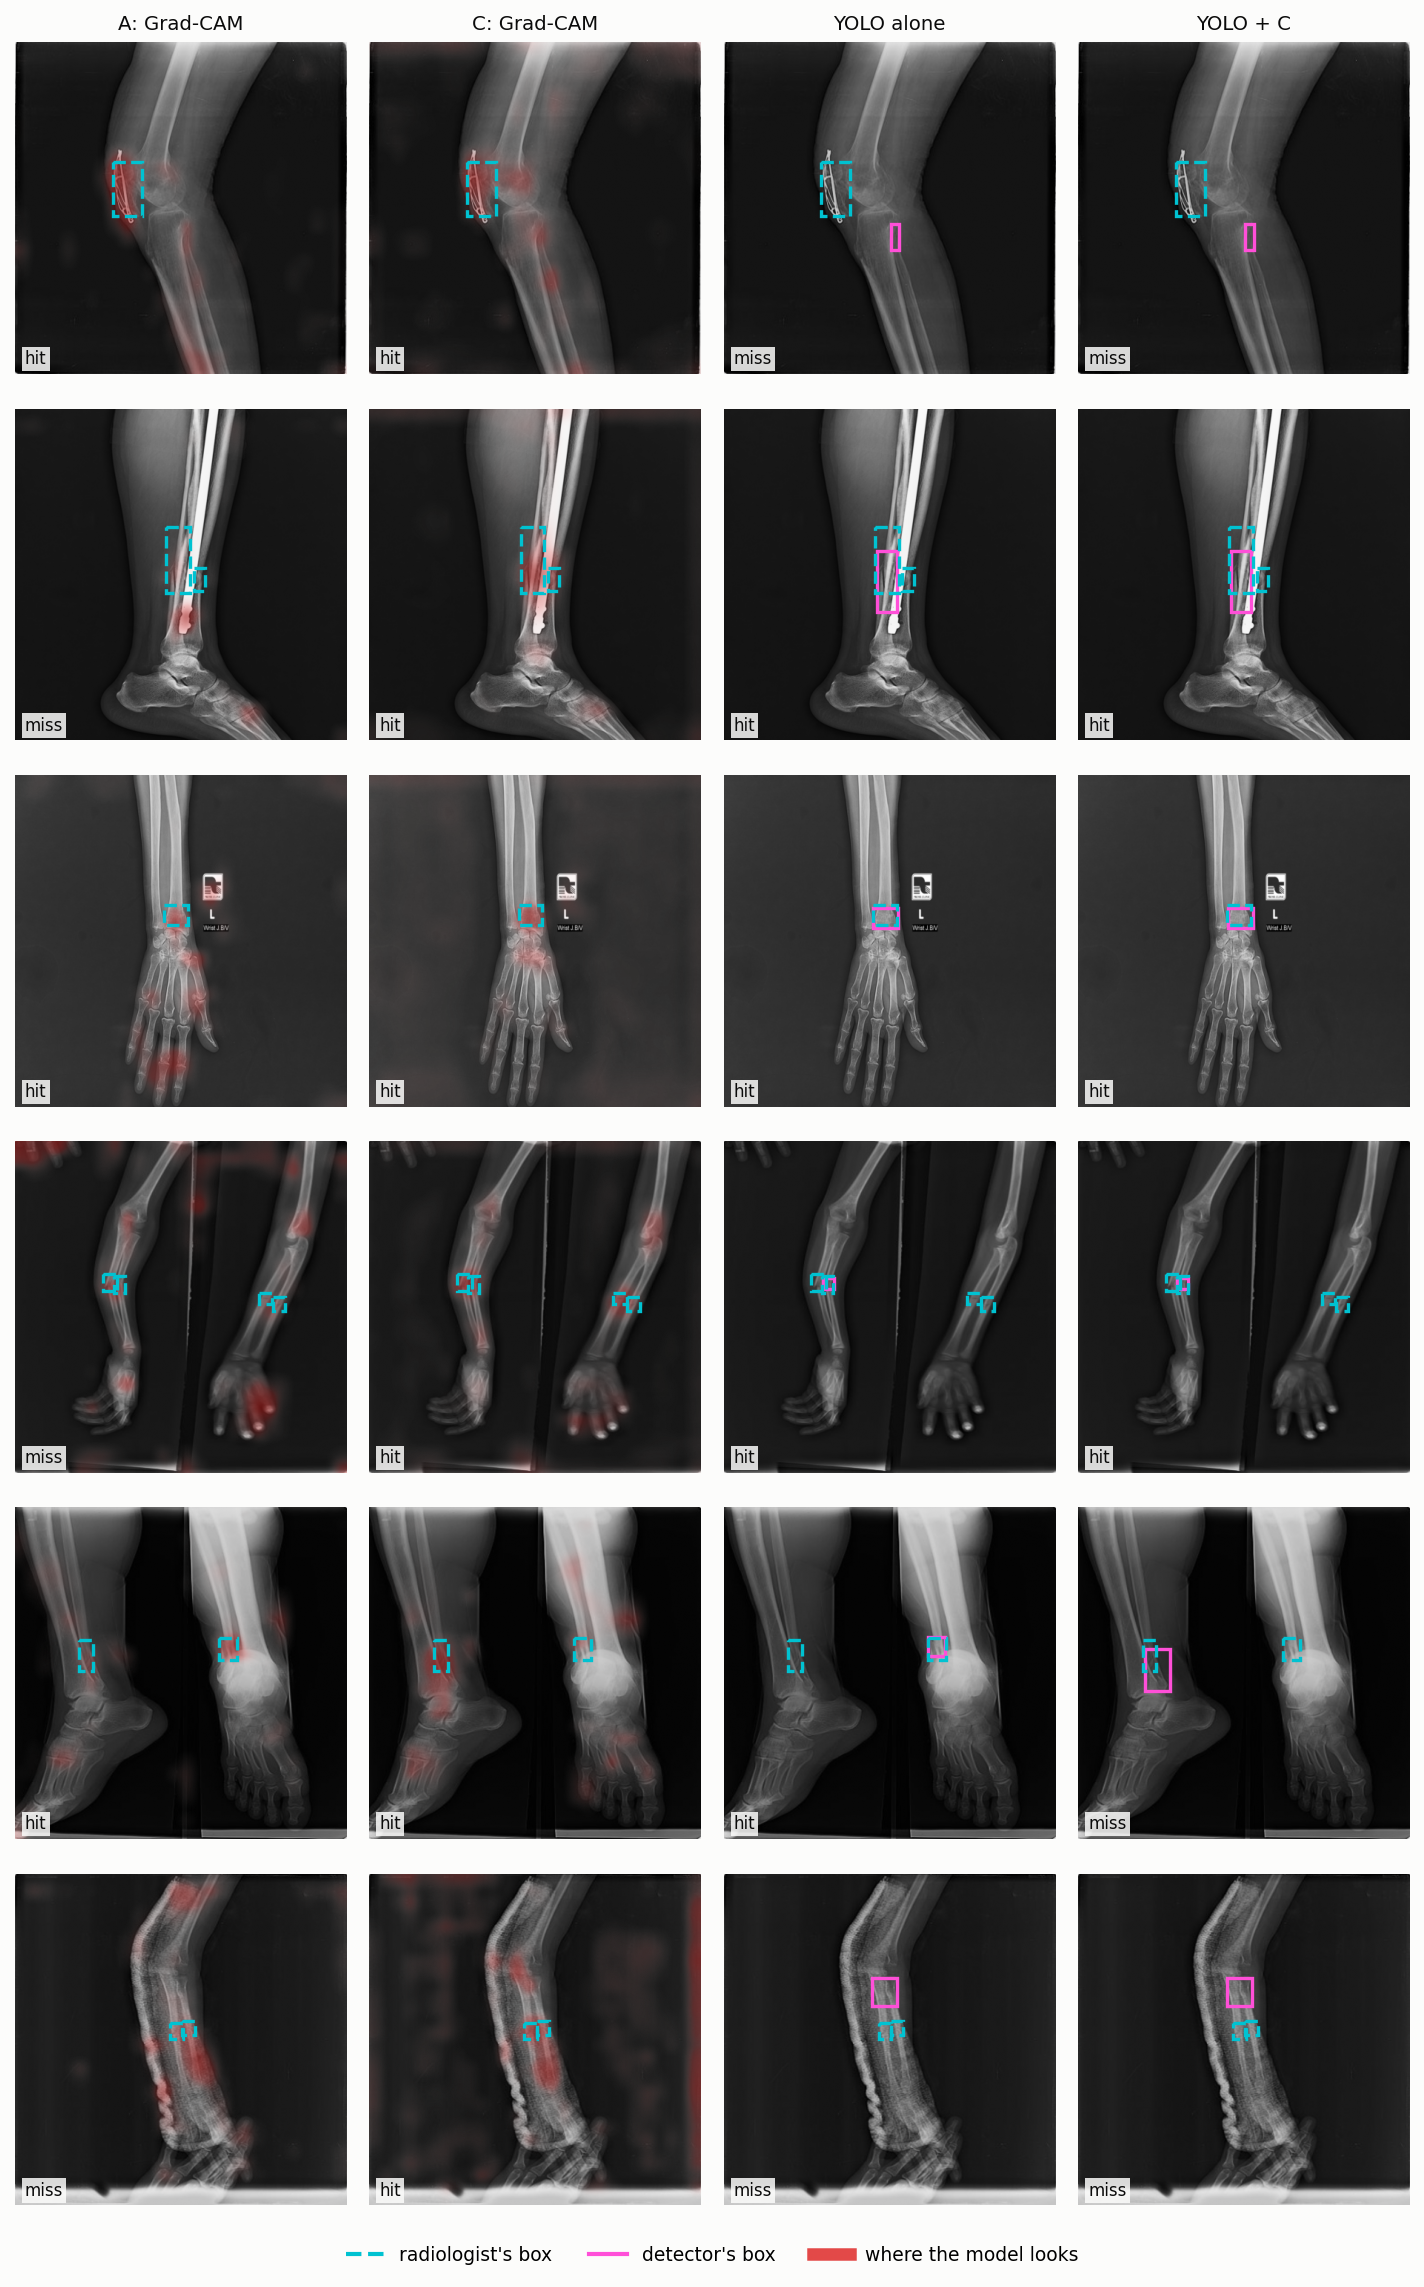
\includegraphics[height=0.82\textheight]{test_gallery.png}
      \end{figure}
    \end{column}
    \begin{column}{0.58\textwidth}
      \small
      \begin{itemize}
        \item Six fractured test X-rays drawn at random.
        \item Columns 1--2: where \textbf{A} and \textbf{C} look (red); dashed: the radiologist's box.
        \item C's evidence is \textbf{tighter} and sits on the bone near the break; A's spreads over the hand, joints
              and edges.
        \item Columns 3--4: YOLO's box, and the box C chooses among YOLO's boxes (next slides).
      \end{itemize}
    \end{column}
  \end{columns}
\end{frame}

\begin{frame}{Can Our Model Help YOLO? YOLO Proposes, C Decides}
  \begin{columns}[T]
    \begin{column}{0.5\textwidth}
      \centering
      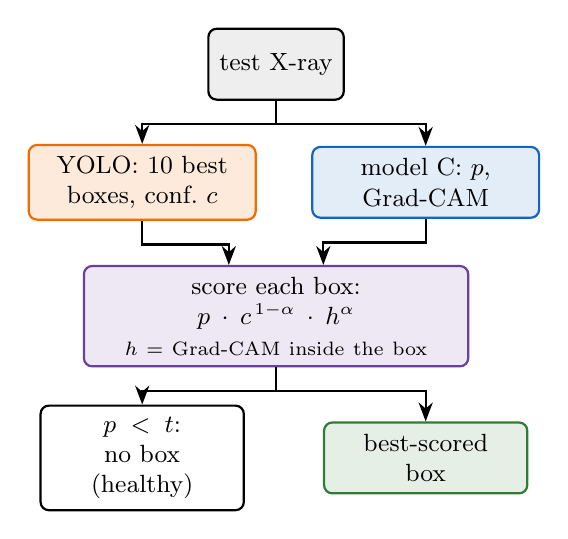
\begin{tikzpicture}[font=\small]
        \node[box] (x) at (0,0) {test X-ray};
        \node[orangebox, text width=2.6cm] (y) at (-1.7,-1.5) {YOLO: 10 best\\boxes, conf.\ $c$};
        \node[bluebox, text width=2.6cm] (m) at (1.9,-1.5) {model C: $p$,\\Grad-CAM};
        \node[violetbox, text width=4.6cm] (s) at (0,-3.2) {score each box:\\$p\cdot c^{\,1-\alpha}\cdot h^{\alpha}$\\\scriptsize $h$ = Grad-CAM inside the box};
        \node[box, fill=white, text width=2.3cm] (d1) at (-1.7,-5.0) {$p<t$:\\no box (healthy)};
        \node[greenbox, text width=2.3cm] (d2) at (1.9,-5.0) {best-scored\\box};
        \draw[arr] (x.south) -- ++(0,-0.3) -| (y.north); \draw[arr] (x.south) -- ++(0,-0.3) -| (m.north);
        \draw[arr] (y.south) -- ++(0,-0.3) -| ([xshift=-6mm]s.north); \draw[arr] (m.south) -- ++(0,-0.3) -| ([xshift=6mm]s.north);
        \draw[arr] (s.south) -- ++(0,-0.3) -| (d1.north); \draw[arr] (s.south) -- ++(0,-0.3) -| (d2.north);
      \end{tikzpicture}
    \end{column}
    \begin{column}{0.48\textwidth}
      \small
      \textbf{YOLOv8s} (COCO-pretrained, 640 px): mAP@0.5 = \textbf{54.4\%} (FracAtlas paper: 56.2\%); its best box is
      on the fracture for \textbf{79\%} of the X-rays: better than any explanation (67\%).
      \vspace{0.4em}

      \textbf{Idea}: YOLO is good at drawing boxes, C at knowing \emph{whether} and \emph{where}.
      \begin{itemize}
        \item $\alpha$ chosen on val: $0.5$ (74.5\% vs 71.6\% for YOLO's order).
        \item $\alpha=0$ is YOLO's own order.
        \item Option: drop the boxes of X-rays C calls healthy.
      \end{itemize}
    \end{column}
  \end{columns}
\end{frame}

\begin{frame}{YOLO vs YOLO + C}
  \begin{columns}[T]
    \begin{column}{0.55\textwidth}
      \begin{figure}
        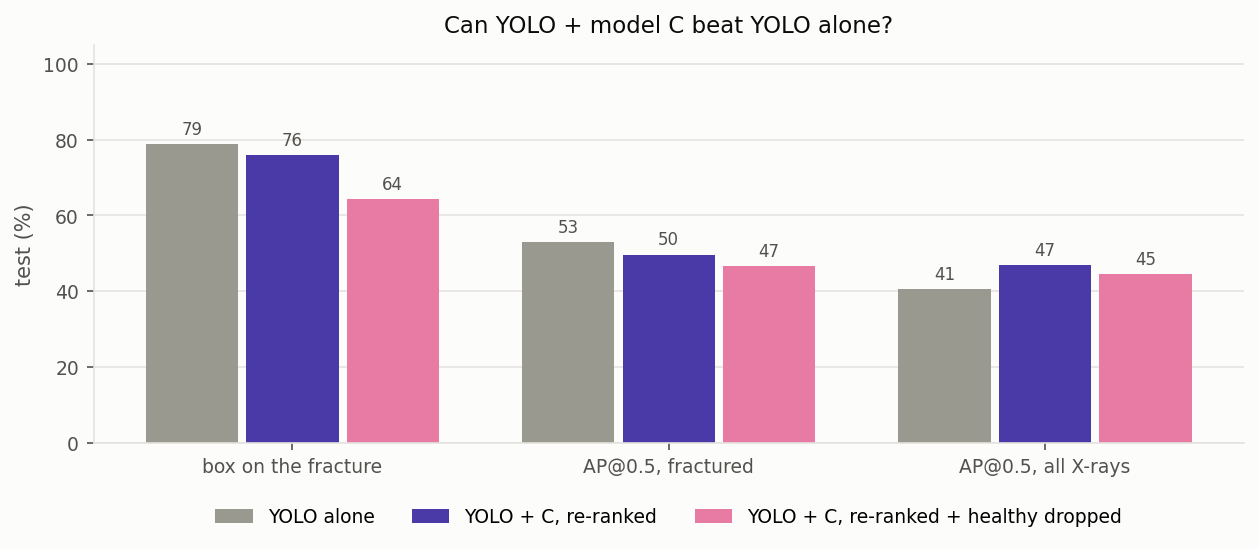
\includegraphics[width=\linewidth]{fusion_scores.png}
      \end{figure}
      \centering\footnotesize
      \begin{tabular}{lcccc}
        \toprule
        & hit & $p$ & AP frac. & AP all \\
        \midrule
        YOLO alone & \textbf{78.8} & -- & \textbf{53.0} & 40.7 \\
        YOLO + C, re-ranked & 76.0 & 0.38 & 49.7 & \textbf{46.9} \\
        \ + healthy dropped & 64.4 & $<$0.001 & 46.6 & 44.6 \\
        \bottomrule
      \end{tabular}
    \end{column}
    \begin{column}{0.43\textwidth}
      \small
      \textbf{Placing the box: no.} 76\% vs 79\%, not significant. YOLO's ranking is already good, and C's Grad-CAM
      (16-px cells) is coarser than YOLO's boxes.
      \vspace{0.4em}

      \textbf{Fewer false boxes: yes.} On all X-rays, AP@0.5 rises from 40.7 to \textbf{46.9}: multiplying by
      $p(\text{fractured})$ pushes YOLO's boxes on healthy X-rays to the bottom.
      \vspace{0.4em}

      \textbf{Dropping boxes} is worse: C misses about 1 fracture in 5.
      \vspace{0.4em}

      $\Rightarrow$ For \emph{where}, use YOLO; for \emph{whether}, use C.
    \end{column}
  \end{columns}
\end{frame}

\begin{frame}{The Pipeline: Two Opinions}
  \begin{columns}[T]
    \begin{column}{0.47\textwidth}
      \centering
      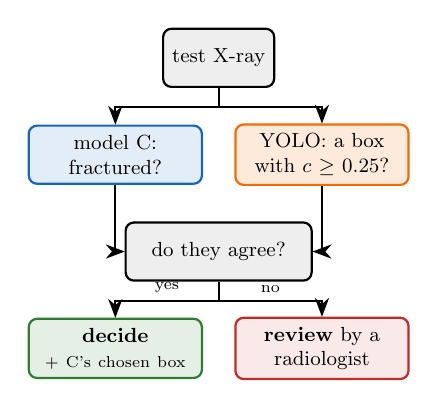
\begin{tikzpicture}[font=\small, scale=0.82, every node/.style={transform shape}]
        \node[box] (x) at (0,0) {test X-ray};
        \node[bluebox, text width=2.4cm] (c) at (-1.6,-1.5) {model C:\\fractured?};
        \node[orangebox, text width=2.4cm] (y) at (1.6,-1.5) {YOLO: a box\\with $c\ge0.25$?};
        \node[box, text width=2.6cm] (q) at (0,-3.0) {do they agree?};
        \node[greenbox, text width=2.4cm] (d) at (-1.6,-4.5) {\textbf{decide}\\\scriptsize + C's chosen box};
        \node[redbox, text width=2.4cm] (r) at (1.6,-4.5) {\textbf{review} by a\\radiologist};
        \draw[arr] (x.south) -- ++(0,-0.3) -| (c.north); \draw[arr] (x.south) -- ++(0,-0.3) -| (y.north);
        \draw[arr] (c.south) |- (q.west); \draw[arr] (y.south) |- (q.east);
        \draw[arr] (q.south) -- ++(0,-0.3) -| node[lab, pos=0.25, above]{yes} (d.north);
        \draw[arr] (q.south) -- ++(0,-0.3) -| node[lab, pos=0.25, above]{no} (r.north);
      \end{tikzpicture}
      \vspace{0.3em}

      \footnotesize
      \begin{tabular}{lc}
        \toprule
        decided & 76\% of the X-rays \\
        right when it decides & \textbf{96.6\%} \\
        sent to review & 24\% \\
        fractures missed & \textbf{5.8\%} (6 of 104) \\
        \bottomrule
      \end{tabular}
    \end{column}
    \begin{column}{0.51\textwidth}
      \begin{figure}
        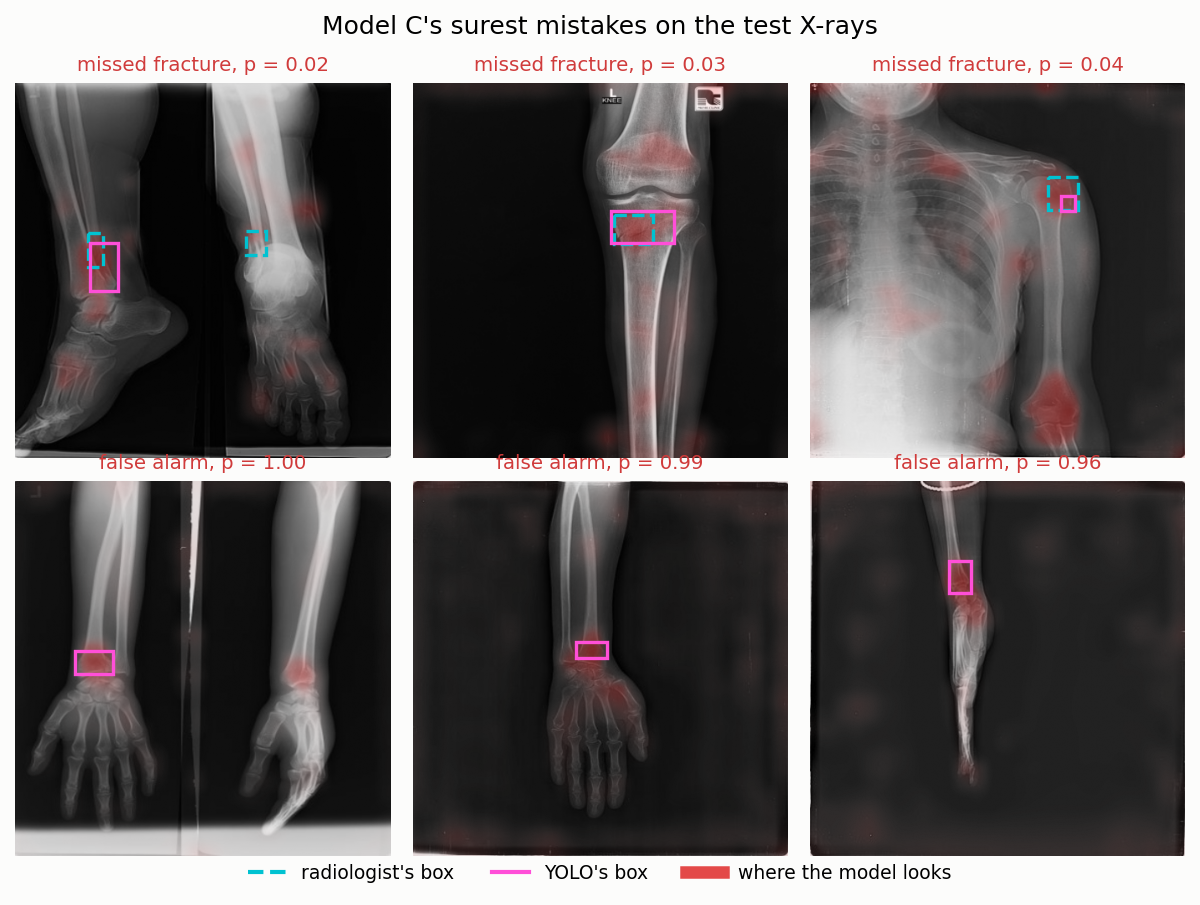
\includegraphics[width=0.78\linewidth]{mistakes.png}
        \caption{C's surest mistakes. Top: missed fractures; bottom: false alarms.}
      \end{figure}
      \vspace{-0.6em}
      \footnotesize On 2 of C's 3 surest \textbf{missed} fractures YOLO's box is \textbf{on} the fracture: the
      pipeline asks for a review instead of missing them.
    \end{column}
  \end{columns}
\end{frame}

\begin{frame}{Every Method Side by Side}
  \centering
  \footnotesize
  \renewcommand{\arraystretch}{1.15}\setlength{\tabcolsep}{4pt}
  \begin{tabular}{>{\raggedright\arraybackslash\bfseries}p{2.2cm}>{\raggedright\arraybackslash}p{4.0cm}ccc>{\raggedright\arraybackslash}p{3.3cm}}
    \toprule
    & \textbf{what it learns} & \textbf{acc.} & \textbf{F1} & \textbf{best hit} & \textbf{good at} \\
    \midrule
    CNN & filters from 2,920 X-rays & 80.9 & 23.3 & 4\% & -- (underfits) \\
    ScatNet & only the classifier & 80.0 & 31.6 & 4\% & stable features, no fractures \\
    ResNet18 & fine-tunes ImageNet & 91.5 & 73.7 & 23\% & classification \\
    A: 448 px & same, 4$\times$ the pixels & 93.3 & 81.0 & 54\% & finding fractures \\
    B: + detector & + where the centre is & \textbf{94.2} & \textbf{82.3} & 60\% & fewest false alarms \\
    \textbf{C: ours} & + where it looks, blur test & 93.0 & 80.4 & \textbf{67\%} & \textbf{looking at the fracture} \\
    YOLOv8 & only boxes & -- & -- & \textbf{79\%} (box) & \textbf{placing the box} \\
    \bottomrule
  \end{tabular}
  \vspace{0.6em}

  \raggedright\small
  ``best hit'': best of the six maps (for YOLO: its most confident box). Same 586 test X-rays for all; A, B, C and
  YOLO at 448--640 px, the others at 224 px.
\end{frame}

\section{Conclusion}

\begin{frame}{Limitations and Lessons}
  \begin{columns}[T]
    \begin{column}{0.49\textwidth}
      \textbf{Limitations}
      \begin{itemize}\small
        \item One dataset; one seed per run (two full runs of A, B, C).
        \item 104 fractured test X-rays: 4 points = 4 X-rays. Deletion test on 10 X-rays.
        \item Loss weights, thresholds, $\alpha$ set once, not tuned.
        \item The pointing game is strict: one point, a tiny box.
        \item C is trained with the blur it is tested with (controls: random patch, five untrained maps).
        \item The built-in detector stays far behind YOLO (AP 22--31\% vs 53\%).
      \end{itemize}
    \end{column}
    \begin{column}{0.47\textwidth}
      \textbf{Lessons}
      \begin{itemize}\small
        \item \textbf{Accuracy is not enough}: 80\% can mean ``finds a fifth of the fractures''.
        \item \textbf{Pretraining and resolution} beat hand-crafted invariance.
        \item A faithful map can still show a \textbf{shortcut}; the model must be \textbf{taught} to look.
        \item \textbf{Score the layer you train}, and test the decision, not only the map.
        \item A \textbf{specialist} stays best at its job: use YOLO for boxes, our model as a second opinion.
      \end{itemize}
    \end{column}
  \end{columns}
\end{frame}

\begin{frame}{Conclusion}
  \begin{itemize}
    \item \textbf{CNN vs ScatNet}: statistically tied and close to ``never fractured''; a pretrained ResNet18 reaches
          \textbf{91.5\%}.
    \item \textbf{Six XAI methods}: the most faithful depends on the model (Grad-CAM for the CNN, LIME for ResNet18);
          our Occlusion equals Captum; but the maps point at the fracture at most \textbf{23\%} of the time.
    \item \textbf{Our joint model} (classifier + detector + explanation losses, 448 px):
      \begin{itemize}
        \item keeps the accuracy (\textbf{93.0\%});
        \item Grad-CAM hits the fracture \textbf{67\%} of the time instead of 35\%;
        \item blurring the fracture now changes the answer (84\% $\to$ \textbf{3\%}).
      \end{itemize}
    \item \textbf{YOLO} remains the best box finder (79\%); our model helps it by removing false boxes (AP on all X-rays
          40.7 $\to$ 46.9), and together they decide 76\% of the X-rays with \textbf{97\%} accuracy.
  \end{itemize}
\end{frame}

\begin{frame}[plain]
  \vfill\centering
  {\usebeamerfont{title}\color{black}Thank you for your attention!\par}
  \vspace{1em}
  {\small Code, results and figures: \texttt{github.com/silvergjeka22/bone-fracture-detection}}
  \vfill
\end{frame}

\end{document}
